\documentclass[10pt]{beamer}
\usepackage{booktabs}
\usepackage{graphicx}
\usepackage{subfigure}
\usepackage{color, colortbl}
\definecolor{Gray}{gray}{0.9}

\title{Authoritarian Regimes}
\author{Session C, Summer 2018}
\date{September 11, 2018}

\begin{document}

\maketitle

\begin{frame}{Democracy in plural societies: Recap}
	Modern society has witnessed two seemingly contradictory political trends.
	\vspace{0.2cm}
	\begin{itemize}
	\item Rise and dominance of nation-states
	\item Repertoire of individual identities and social cleavages
	\end{itemize}
\end{frame}

\begin{frame}{Democracy in plural societies: Recap}
	Plural society emerges when a state	contains competing politicized identities and cleavages.
	\vspace{0.2cm}
	\begin{itemize}
	\item Underdevelopment and poor supply of public goods
	\item Domestic conflicts and civil wars
	\item Discrimination and inequality
	\end{itemize}
\end{frame}

\begin{frame}{Democracy in plural societies: Recap}
	\begin{columns}
	\column{0.5\linewidth}
	Plural societies are plagued by ``mutual antipathies.''
	\vspace{0.2cm}	
	\begin{itemize}
	\item Consensus
	\item Collective action: Cooperation and coordination
	\end{itemize}
	\column{0.4\linewidth}
    \centering
    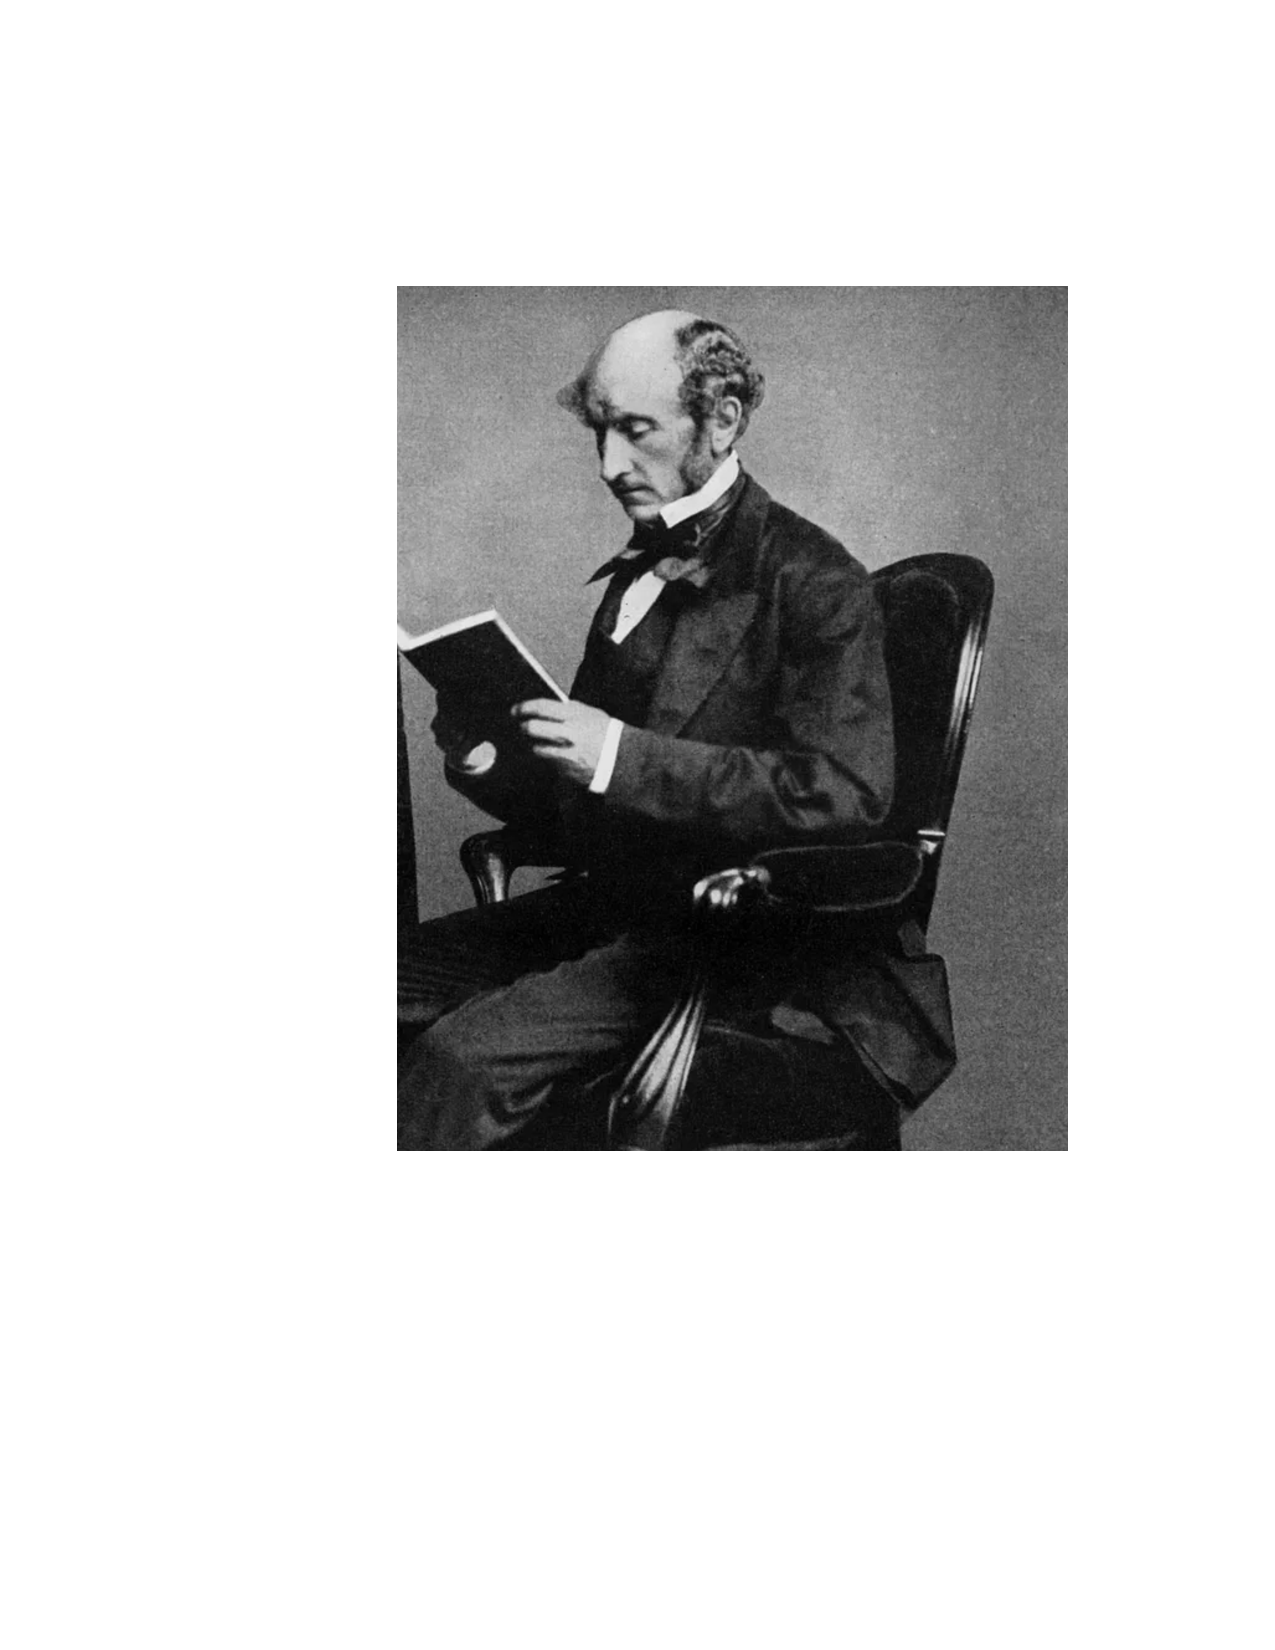
\includegraphics[scale=0.42]{Figs/jsm}
    \end{columns}
\end{frame}

\begin{frame}{Democracy in plural societies: Recap}
	When and how will an identity or social cleavage become politically relevant?
	\vspace{0.2cm}
	\begin{itemize}
	\item History
	\item Local context
	\item Structure of cleavages
	\item Political mobilization (or de-mobilization)
	\item Constitutional design: Consociationalism (?)
	\end{itemize}
\end{frame}

\begin{frame}{Democracy in plural societies: Recap}
	\begin{figure}
	\centering
	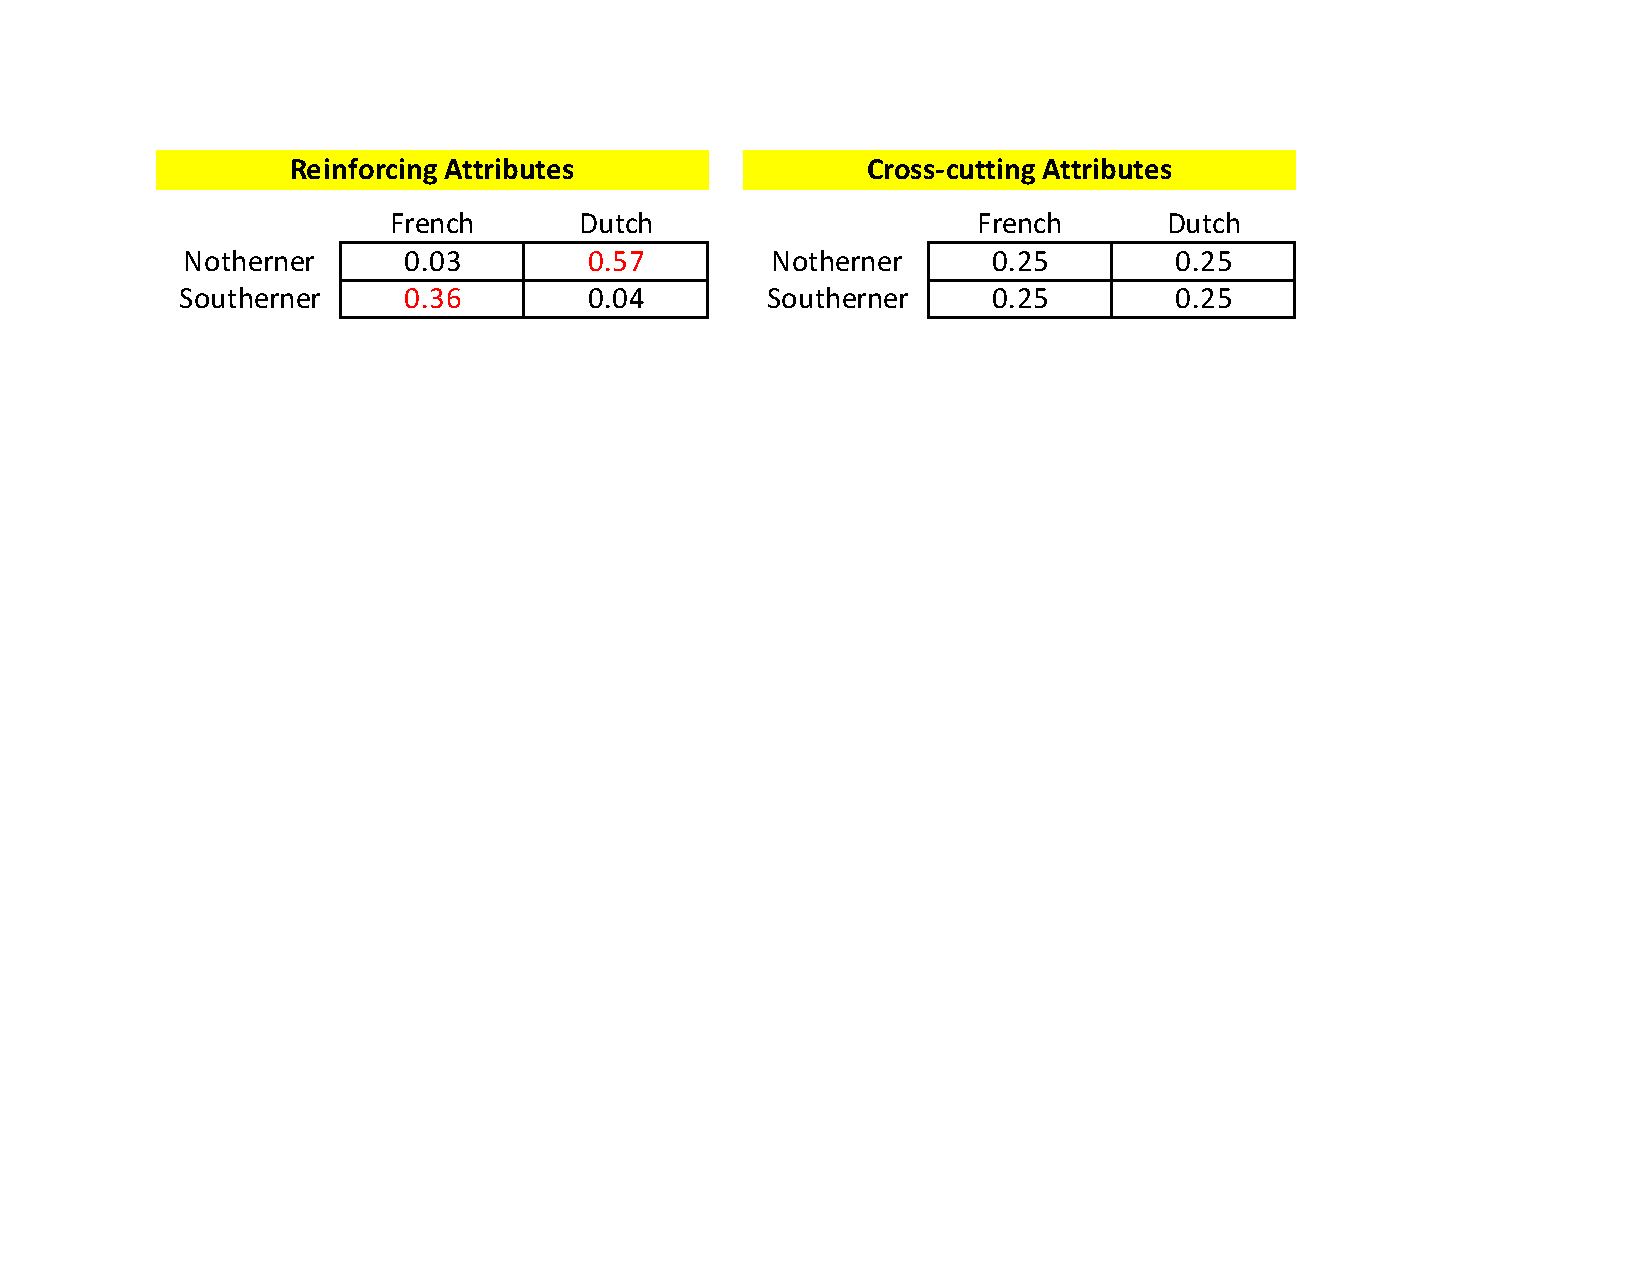
\includegraphics[scale=0.55]{Figs/structure}
	\end{figure}
	\pause
	Politics is more divisive when cleavages are highly correlated.
\end{frame}

\begin{frame}{Democracy in plural societies: Recap}
	How can a state overcome social cleavages to build a united nation?
	\vspace{0.2cm}
	\begin{itemize}
	\item Repression and common enemy
	\item Overarching ideology, common history, and shared language
	\end{itemize}
\end{frame}

\begin{frame}{India: A case of nation building}
	\begin{figure}
	\centering
	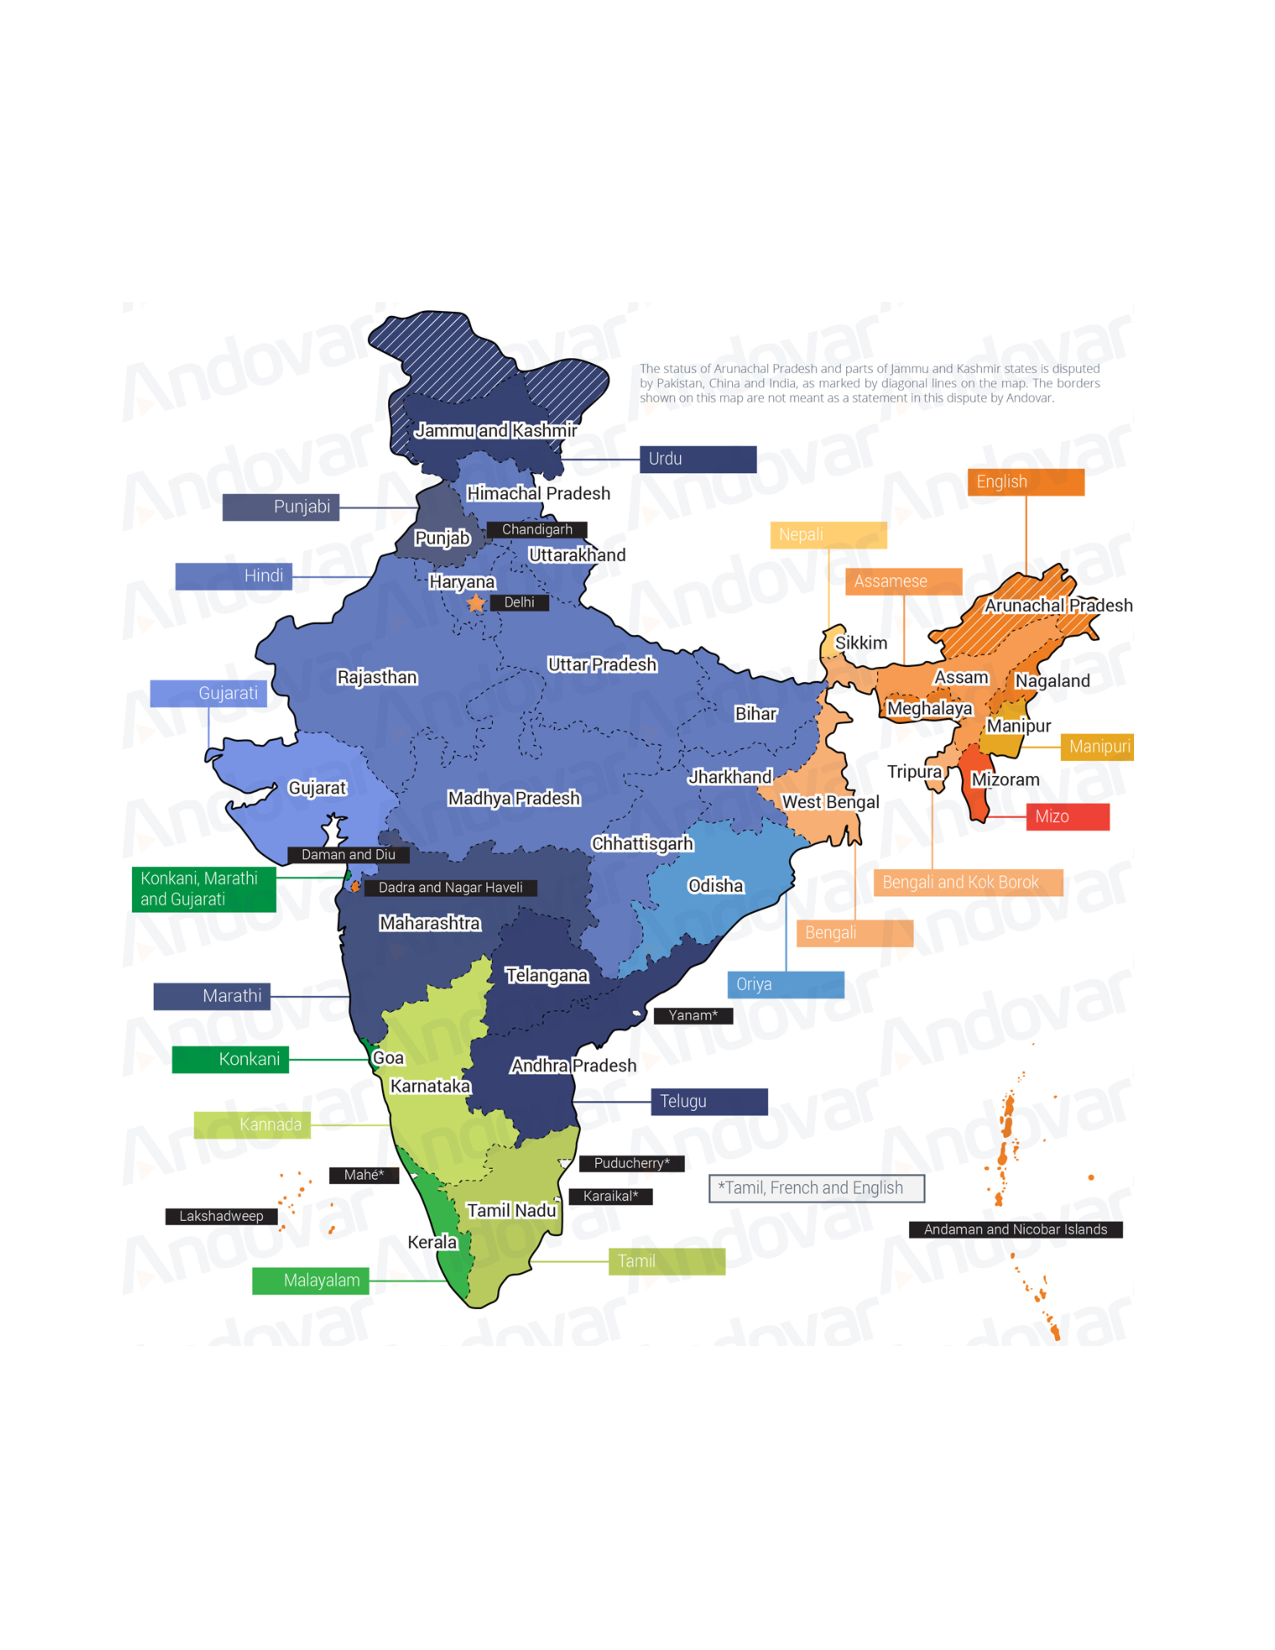
\includegraphics[scale=0.45]{Figs/India/india}
	\end{figure}
\end{frame}

\begin{frame}{India: A case of nation building}
	\begin{figure}
	\centering
	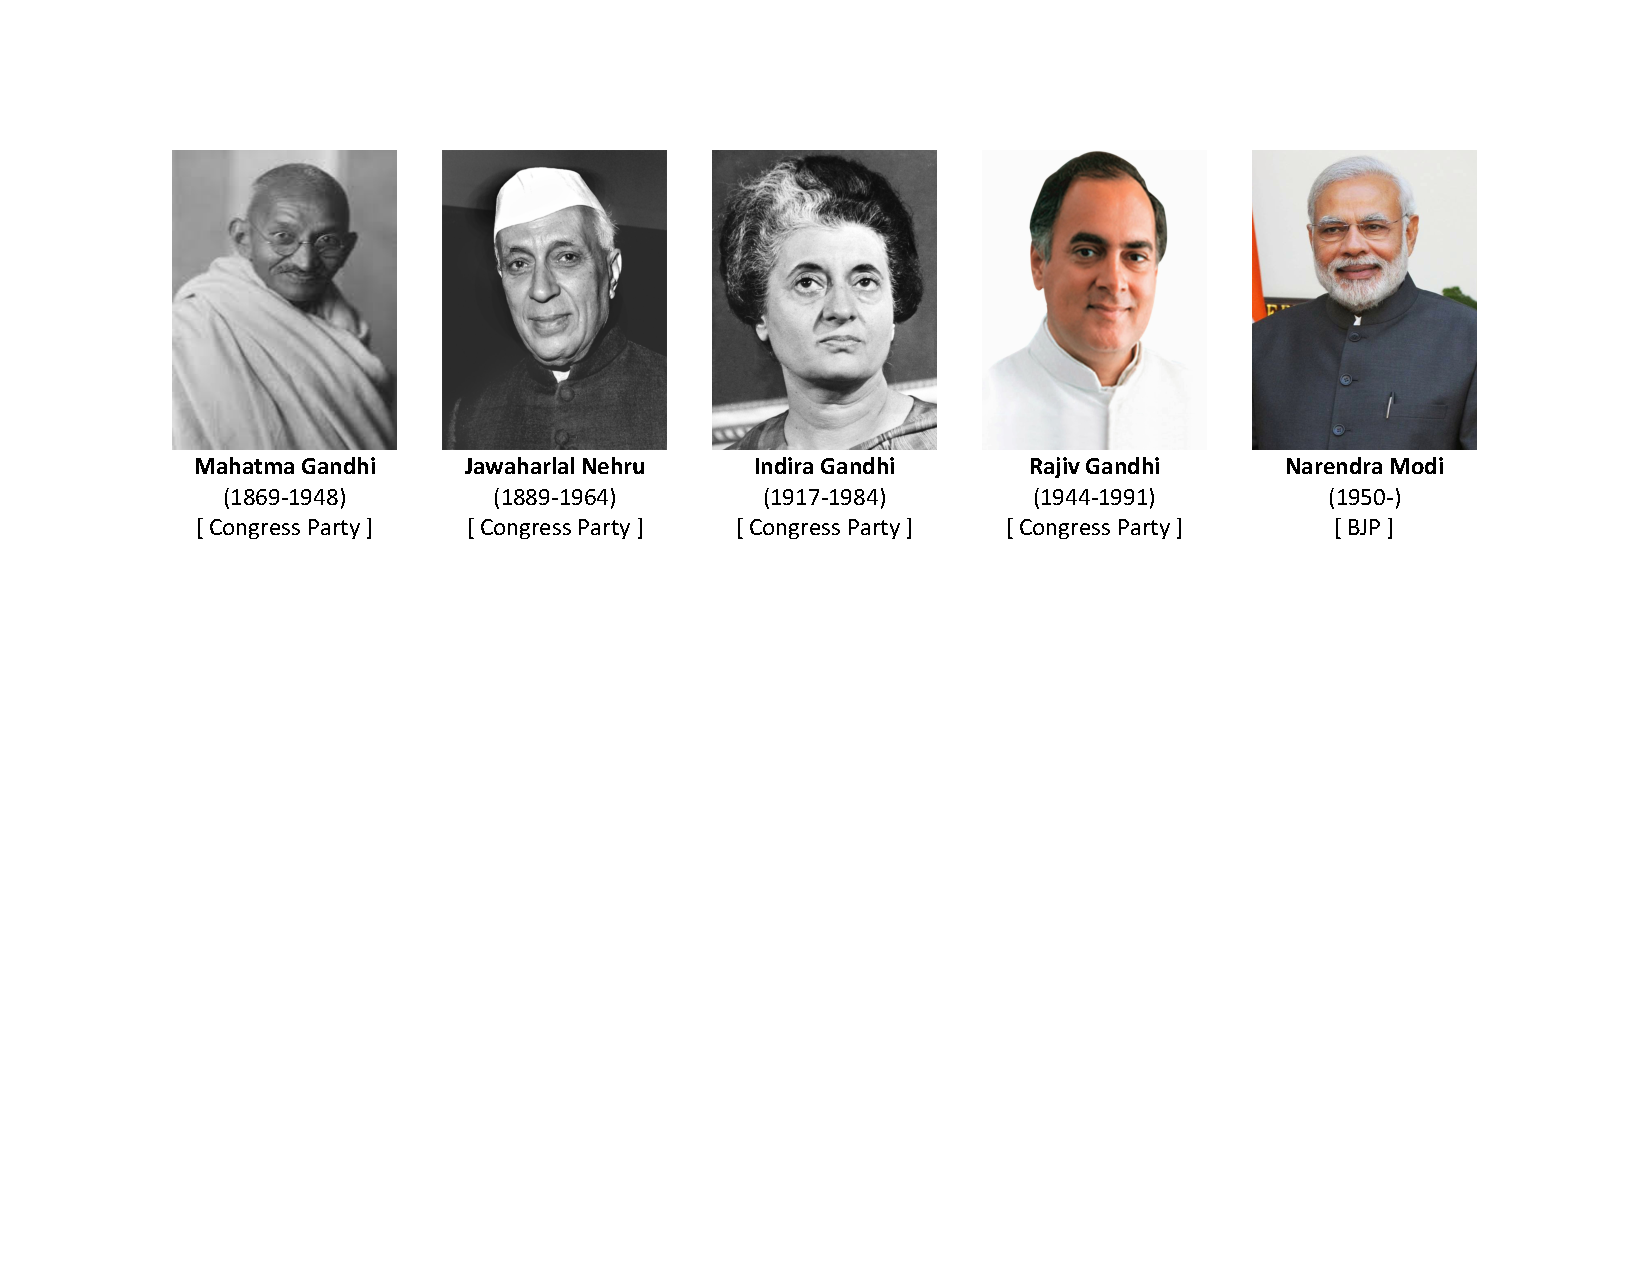
\includegraphics[scale=0.5]{Figs/India/leaders}
	\end{figure}
	\pause
	\begin{itemize}
	\item Congress Party created as a political party of the ``Indian'' nation.
	\item The British colonial rule as the common enemy (?).
	\item The Constitution outlaws discrimination against marginalized groups along with with the provision of political reservations and affirmative action policies.
	\end{itemize}
\end{frame}

\begin{frame}{India: A case of nation building}
	\begin{figure}
	\centering
	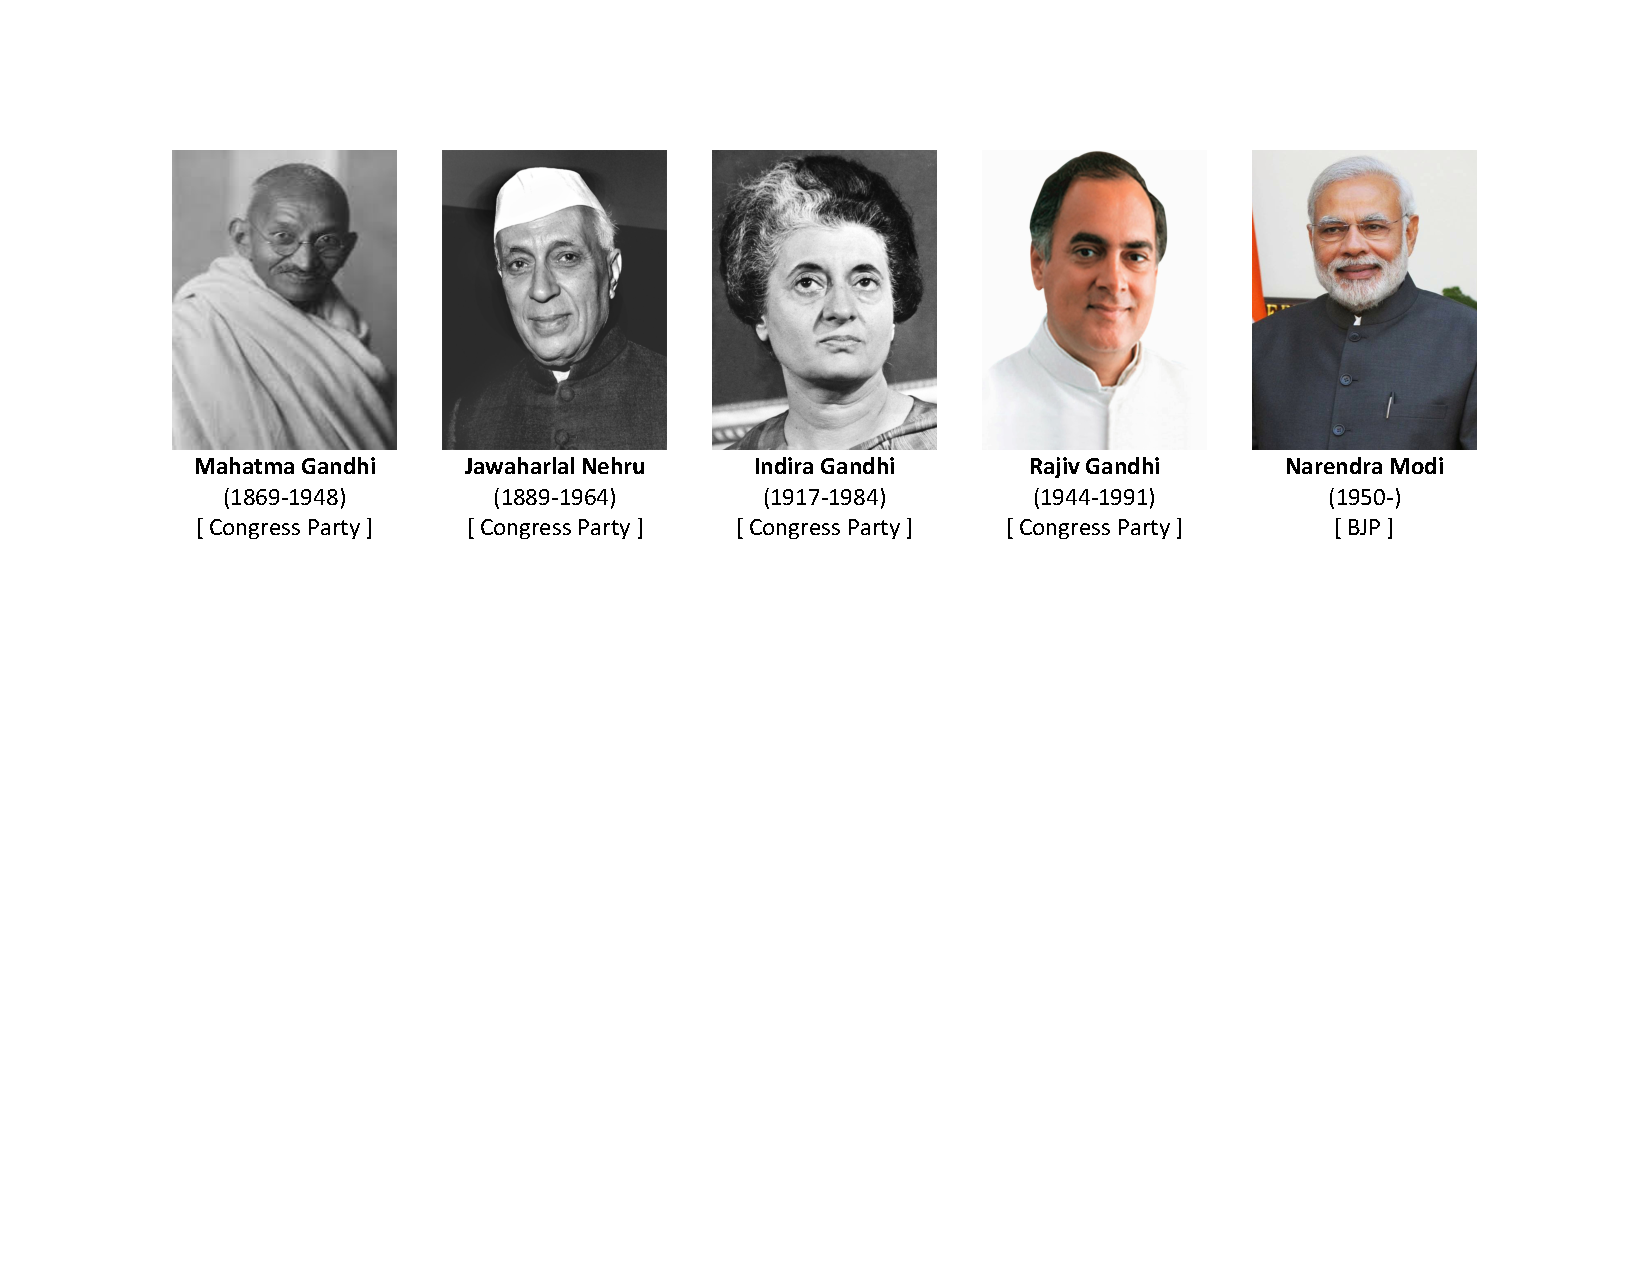
\includegraphics[scale=0.5]{Figs/India/leaders}
	\end{figure}
	\pause
	\begin{itemize}
	\item M. Gandhi assassinated by a supporter of Hindu nationalism.
	\item I. Gandhi assassinated by her Sikh guards after Operation Blue Star.
	\item R. Gandhi assassinated by Liberation Tigers of Tamil Eelam from Sri Lanka.
	\end{itemize}
\end{frame}

\begin{frame}{Today's plan}
	\begin{itemize}
		\item What is an authoritarian regime?
		\item How can we identify an authoritarian regime?
		\item How do authoritarian regimes differ from each other?
		\item How do authoritarian regimes stay in power?
	\end{itemize}
\end{frame}

\begin{frame}{Recent developments in US politics}
	\begin{figure}
	\setcounter{subfigure}{0}
	\footnotesize
	\centering
	\subfigure[July 16, 2018]{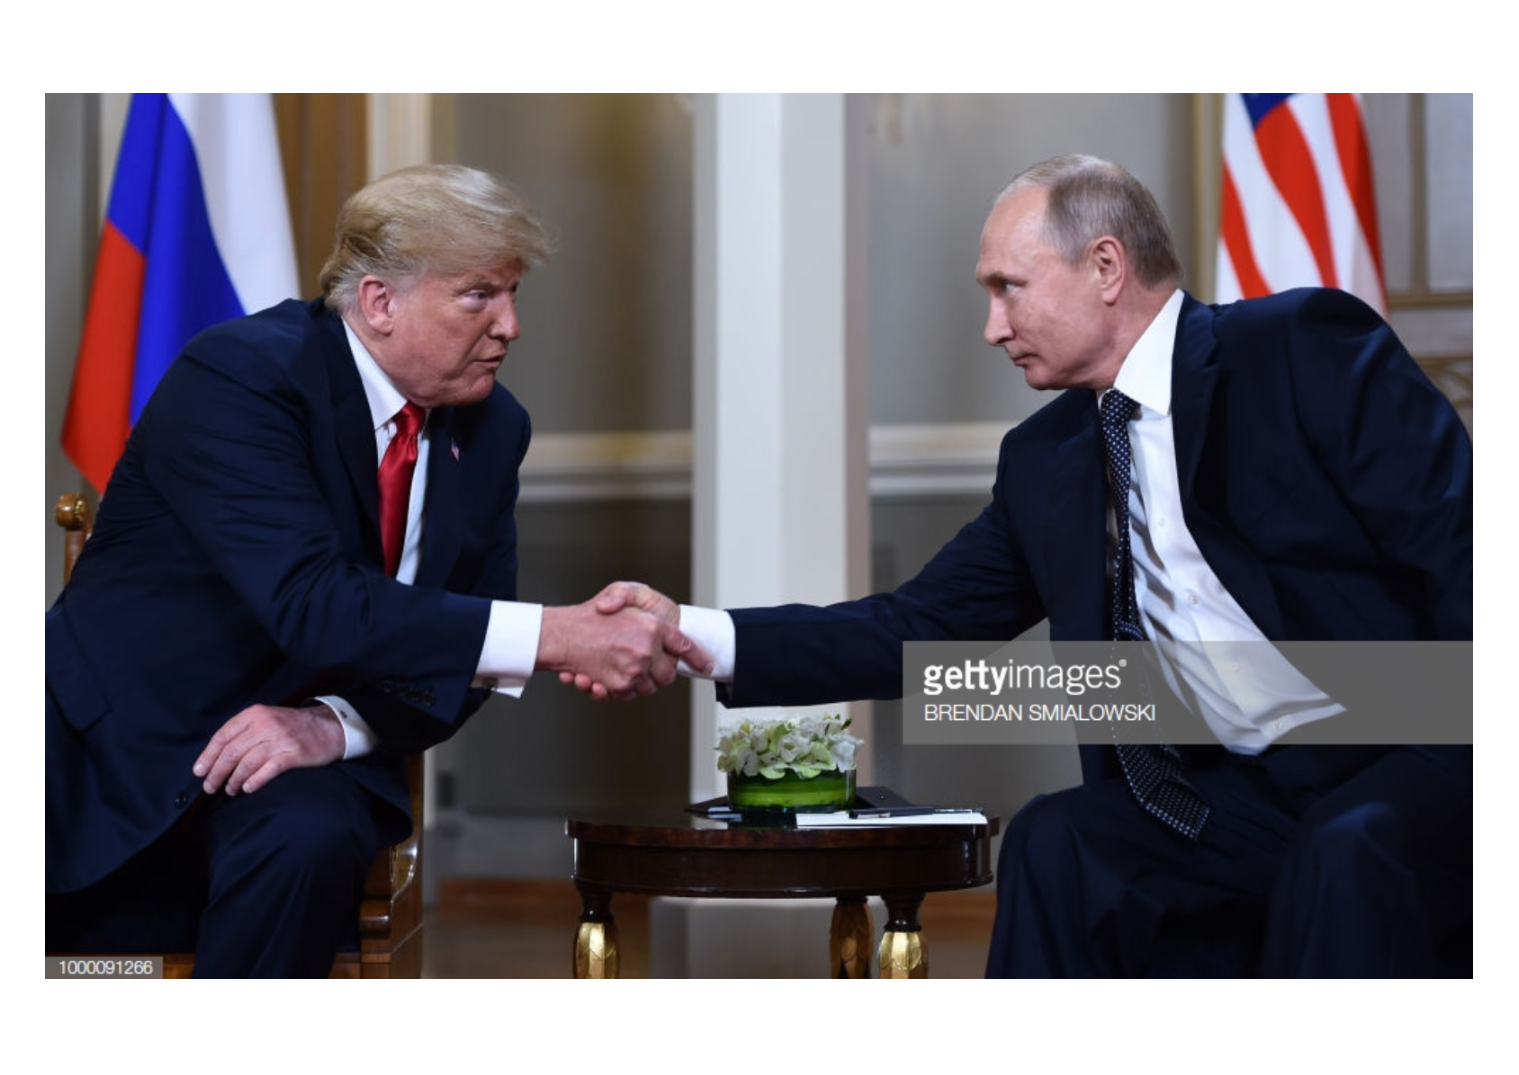
\includegraphics[height=3.3cm,width=5cm]{Figs/USA/trump_putin}}
	\hspace{0.1cm}
	\subfigure[June 12, 2018]{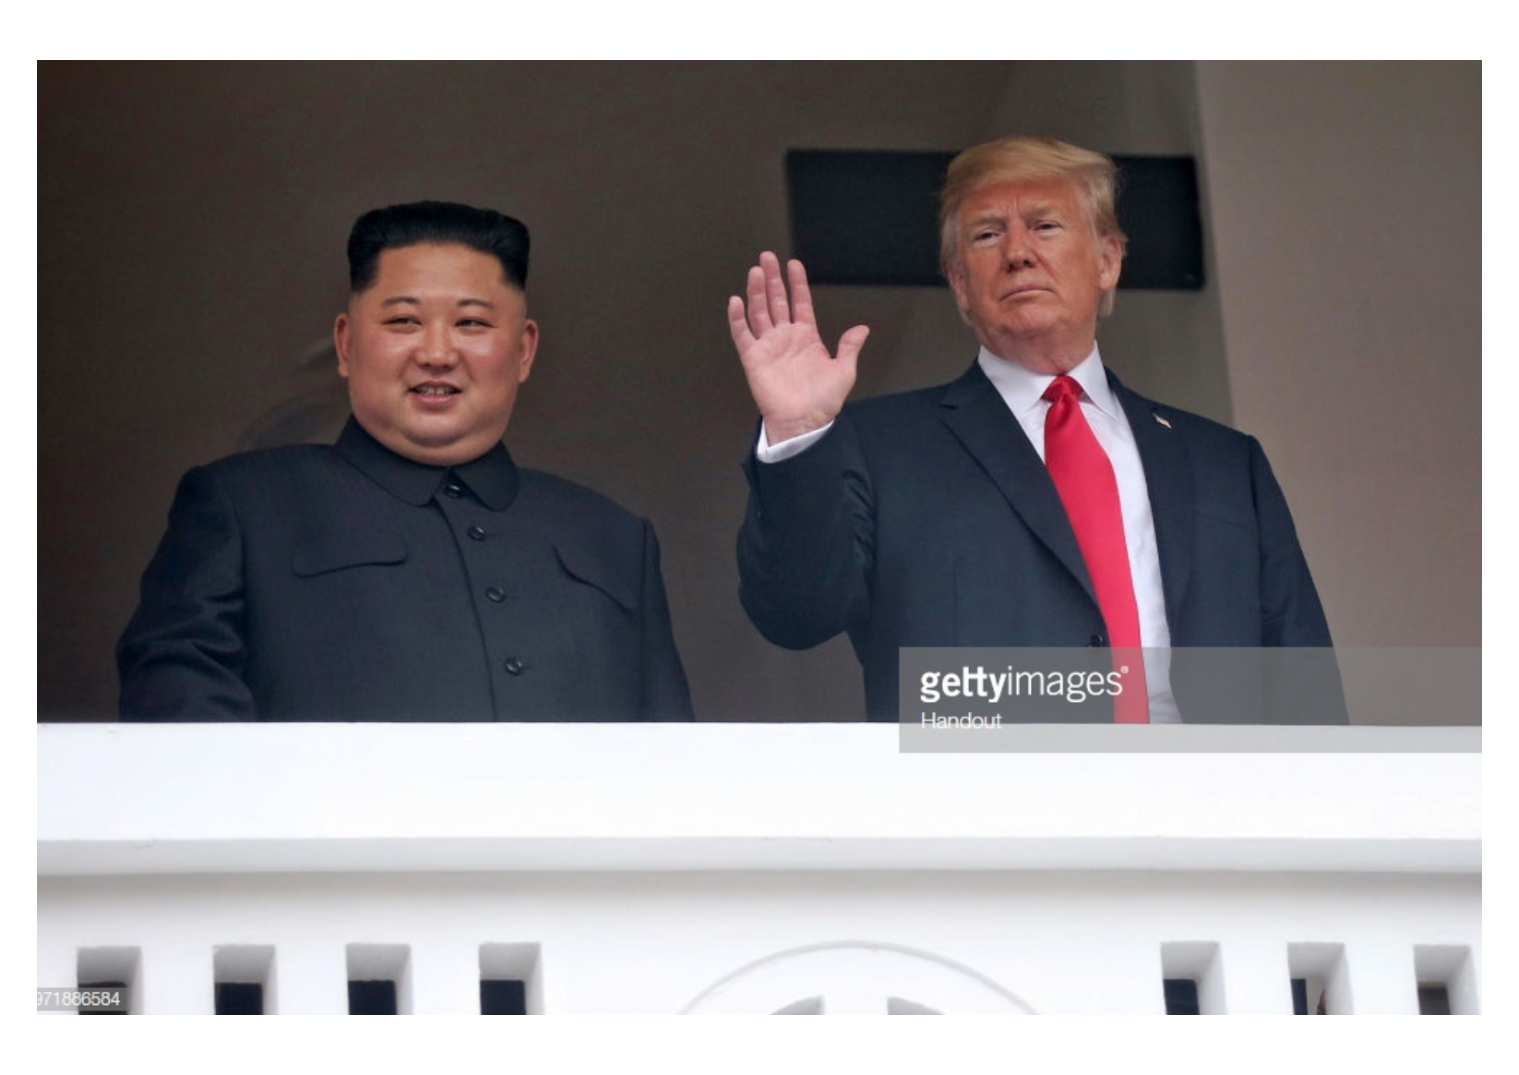
\includegraphics[height=3.3cm,width=5cm]{Figs/USA/trump_kim}}
	\end{figure}
\end{frame}

\begin{frame}{Recent developments in US politics}
	\begin{columns}
    \column{0.5\linewidth}
    \small
	``If he says great things about me, I'm going to say great things about him. I've already said, \textbf{he is really very much of a leader}. I mean, you can say, oh, isn't that a terrible thing -- the man has very strong control over a country. Now, it's a very different system, and I don't happen to like the system. But certainly, in that system, he's been a leader, far more than our president has been a leader.''	\vspace{0.2cm}
    \column{0.42\linewidth}
    \centering
    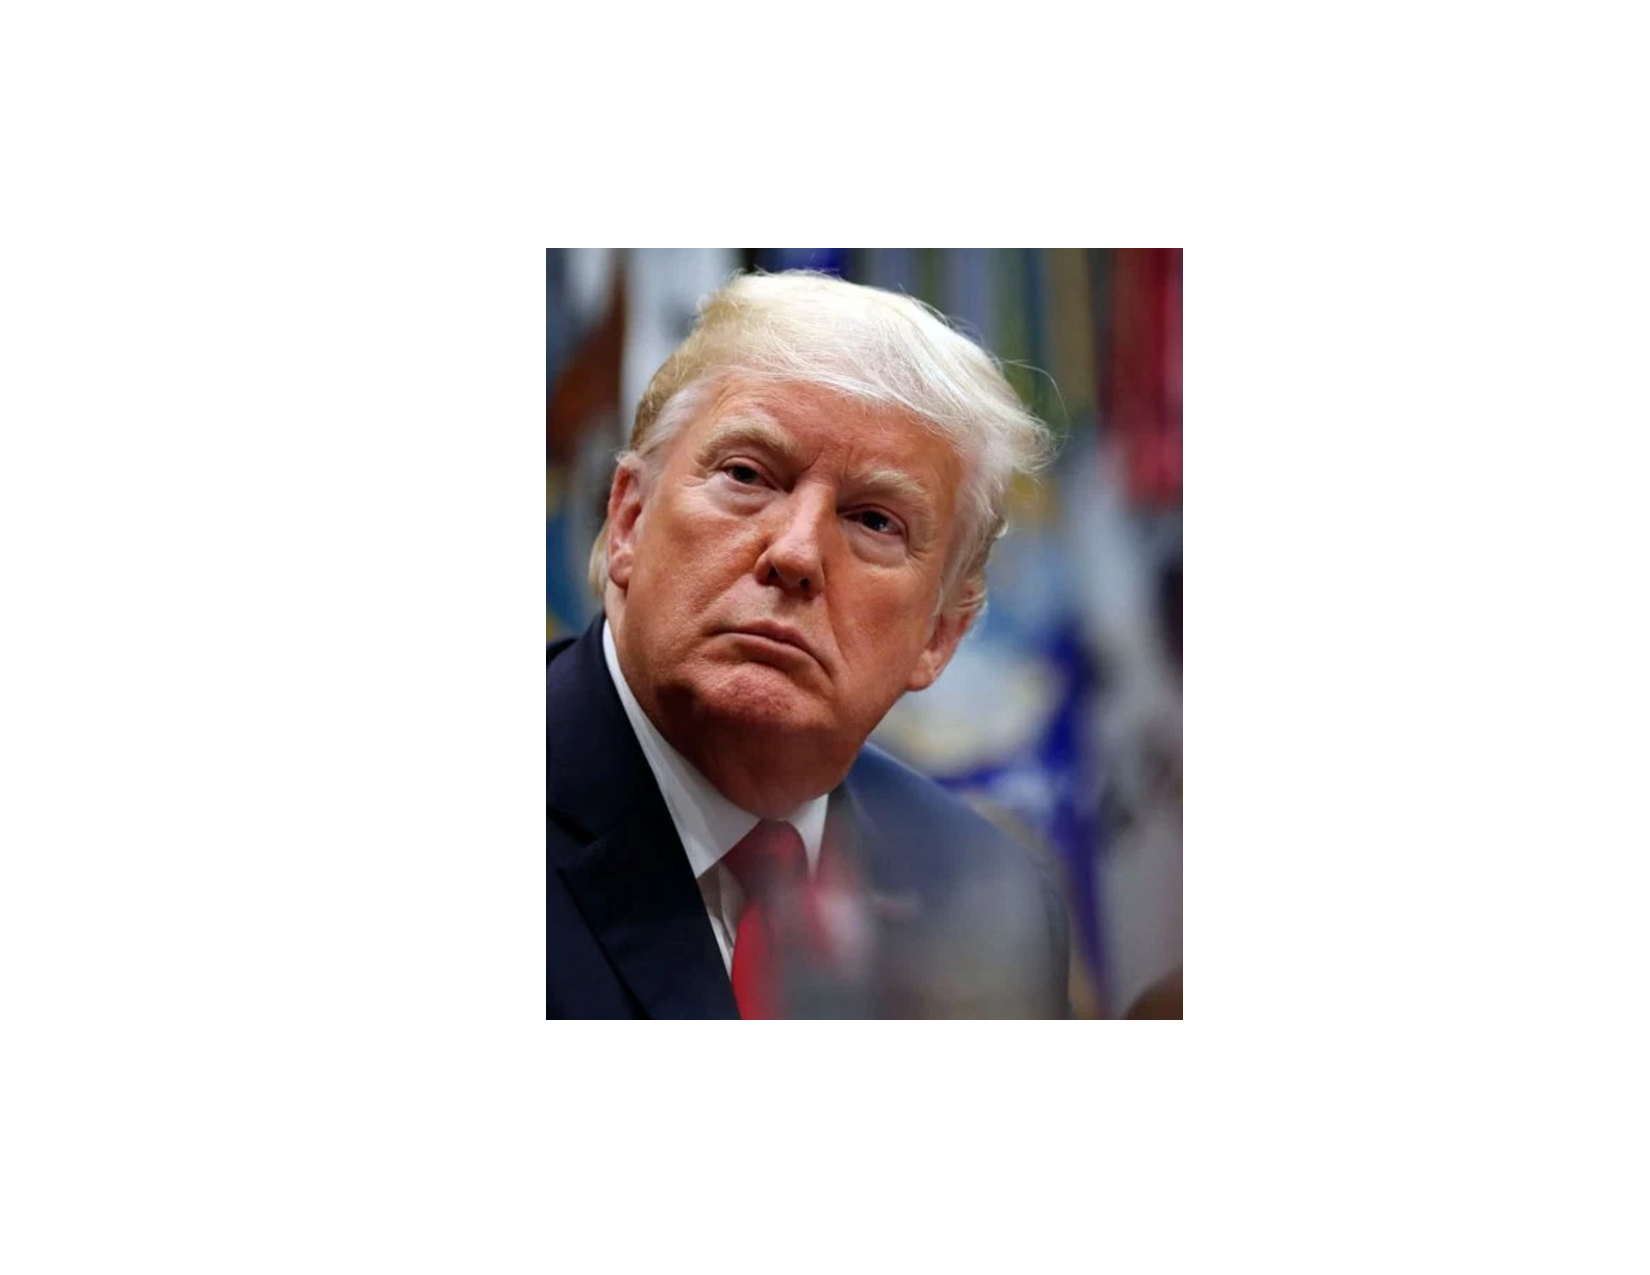
\includegraphics[scale=0.55]{Figs/trump}
    \end{columns}
\end{frame}

\begin{frame}{Recent developments in US politics}
	\begin{figure}
	\centering
	\includegraphics[scale=0.4]{Figs/autocrats}
	\end{figure}
\end{frame}

\begin{frame}{Democracy in crisis?}
	\begin{figure}
	\centering
	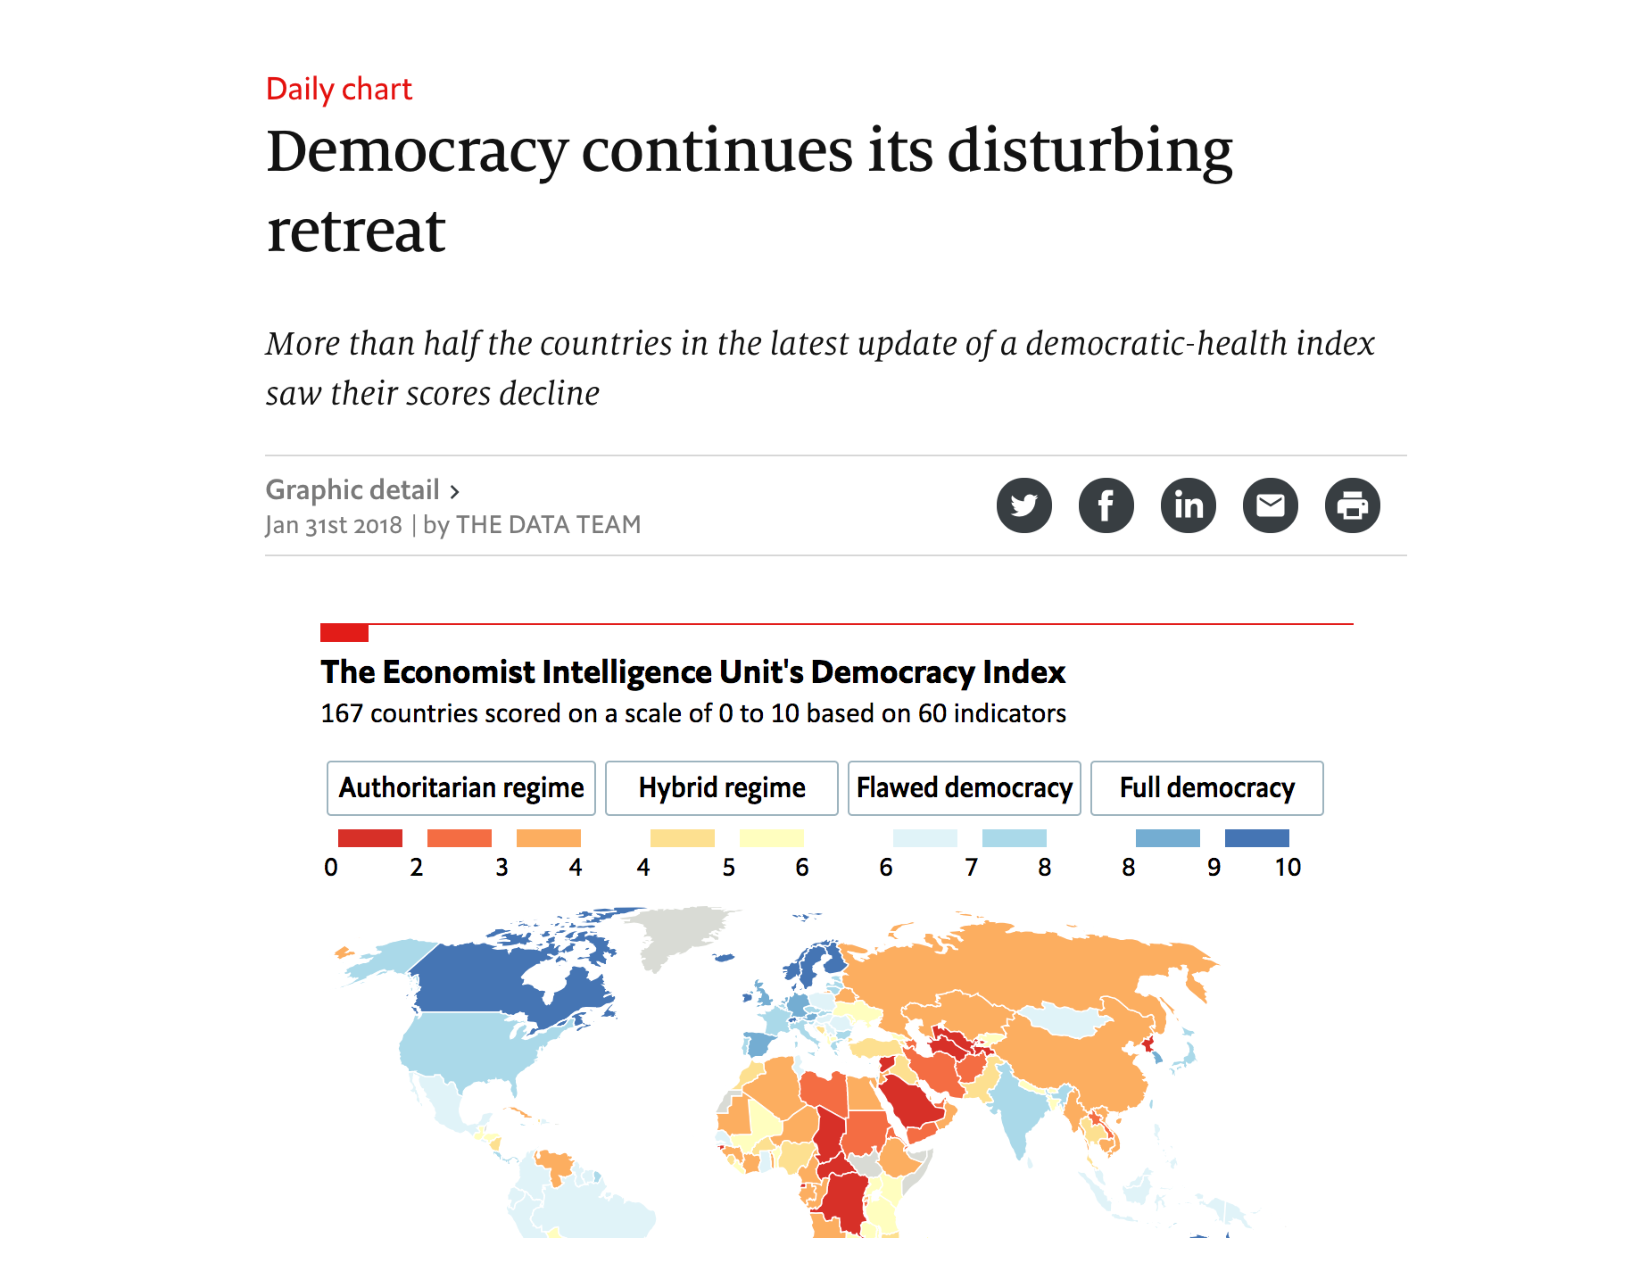
\includegraphics[scale=0.38]{Figs/democracy_retreat}
	\end{figure}
\end{frame}

\begin{frame}{Democracy in crisis?}
	\begin{figure}
	\centering
	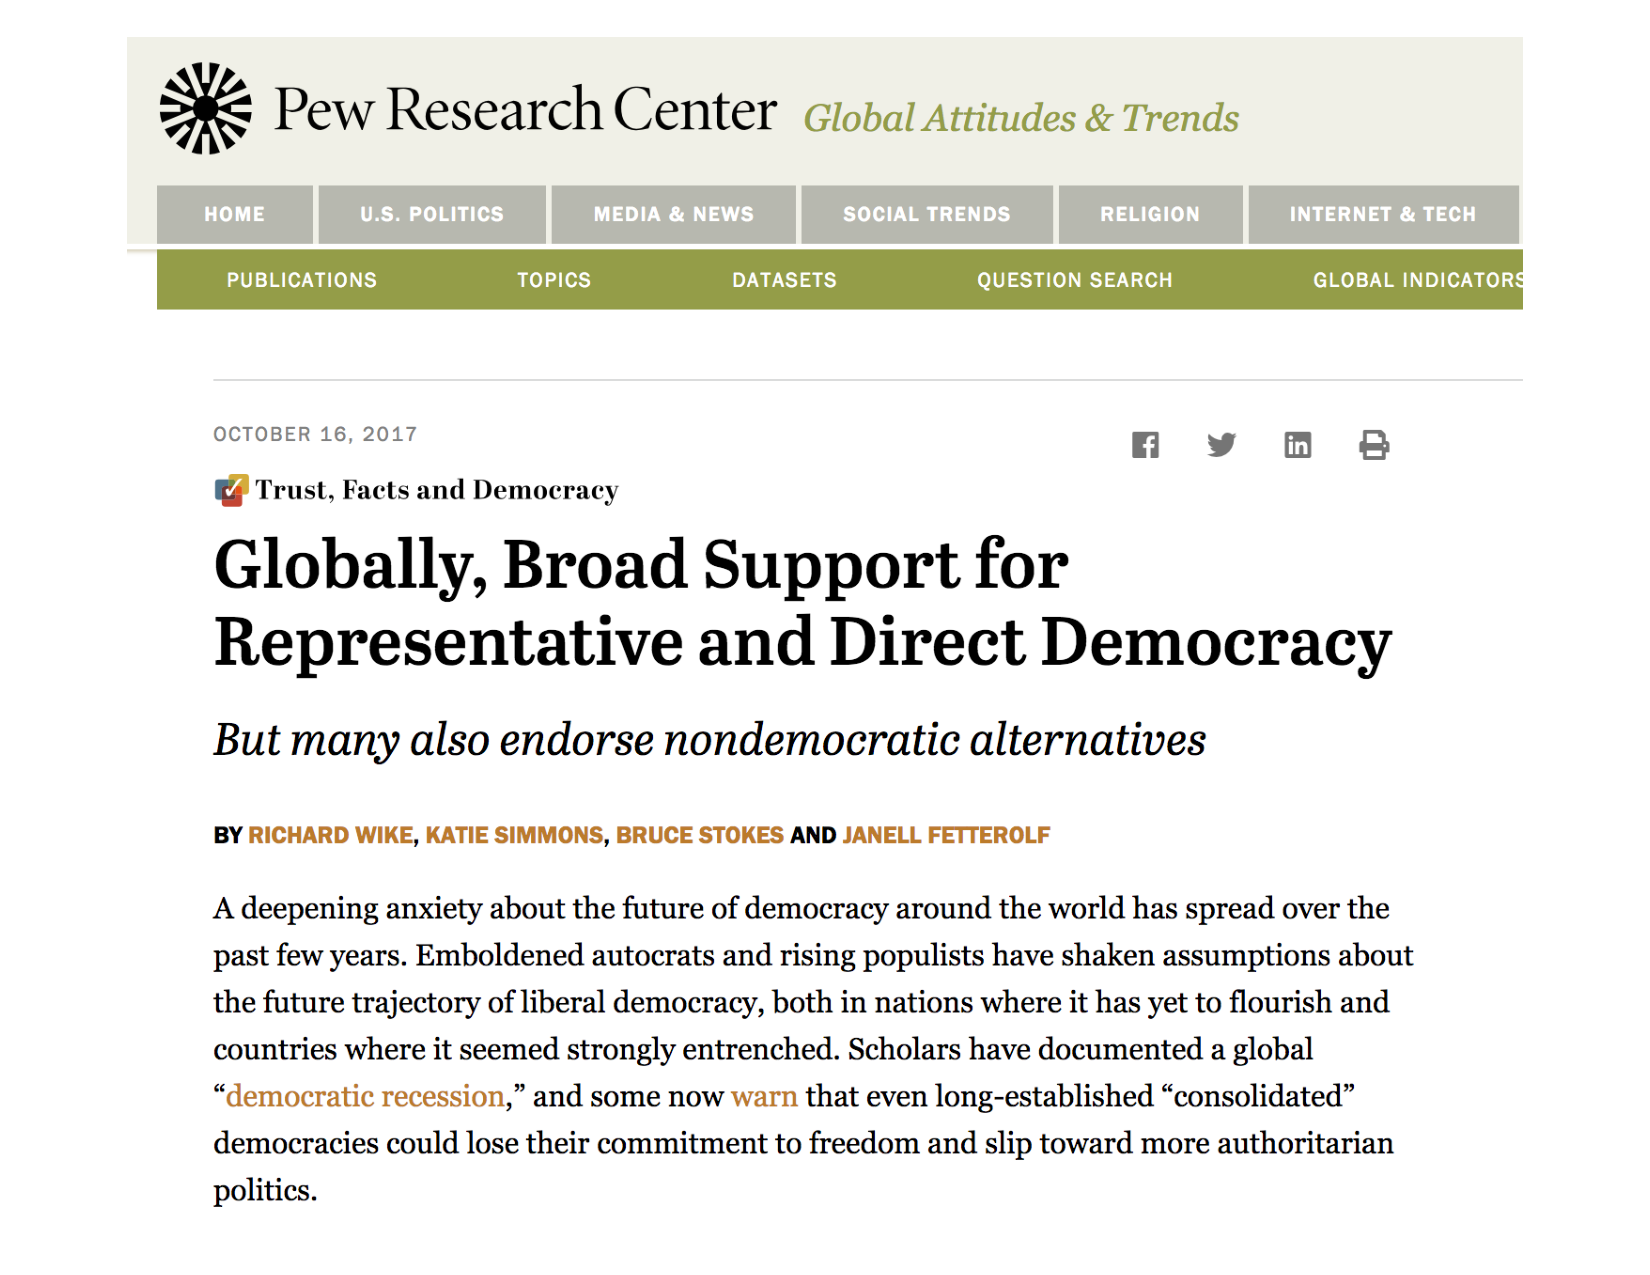
\includegraphics[scale=0.38]{Figs/democracy_support}
	\end{figure}
\end{frame}

\begin{frame}{Democracy in crisis?}
	\begin{figure}
	\centering
	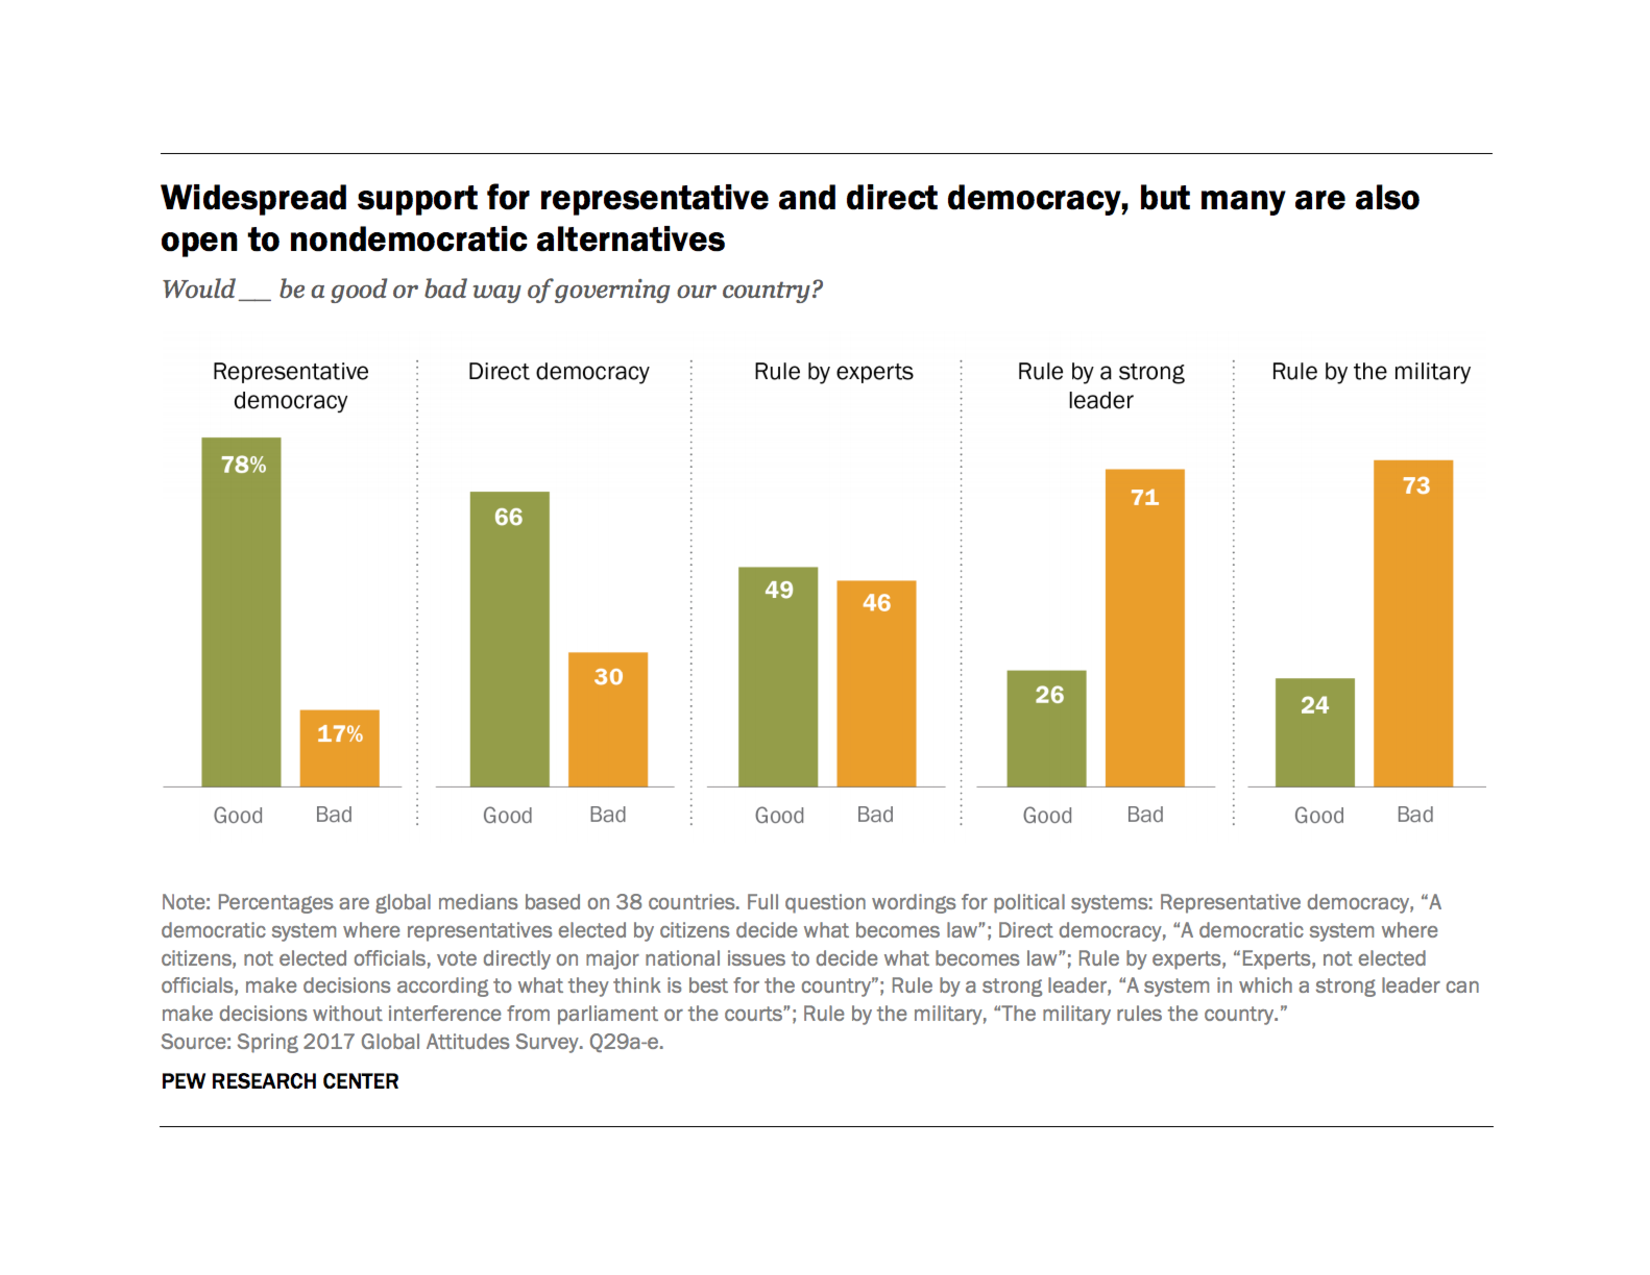
\includegraphics[scale=0.42]{Figs/pew}
	\end{figure}
\end{frame}

\begin{frame}{Democracy in crisis?}
	\begin{figure}
	\centering
	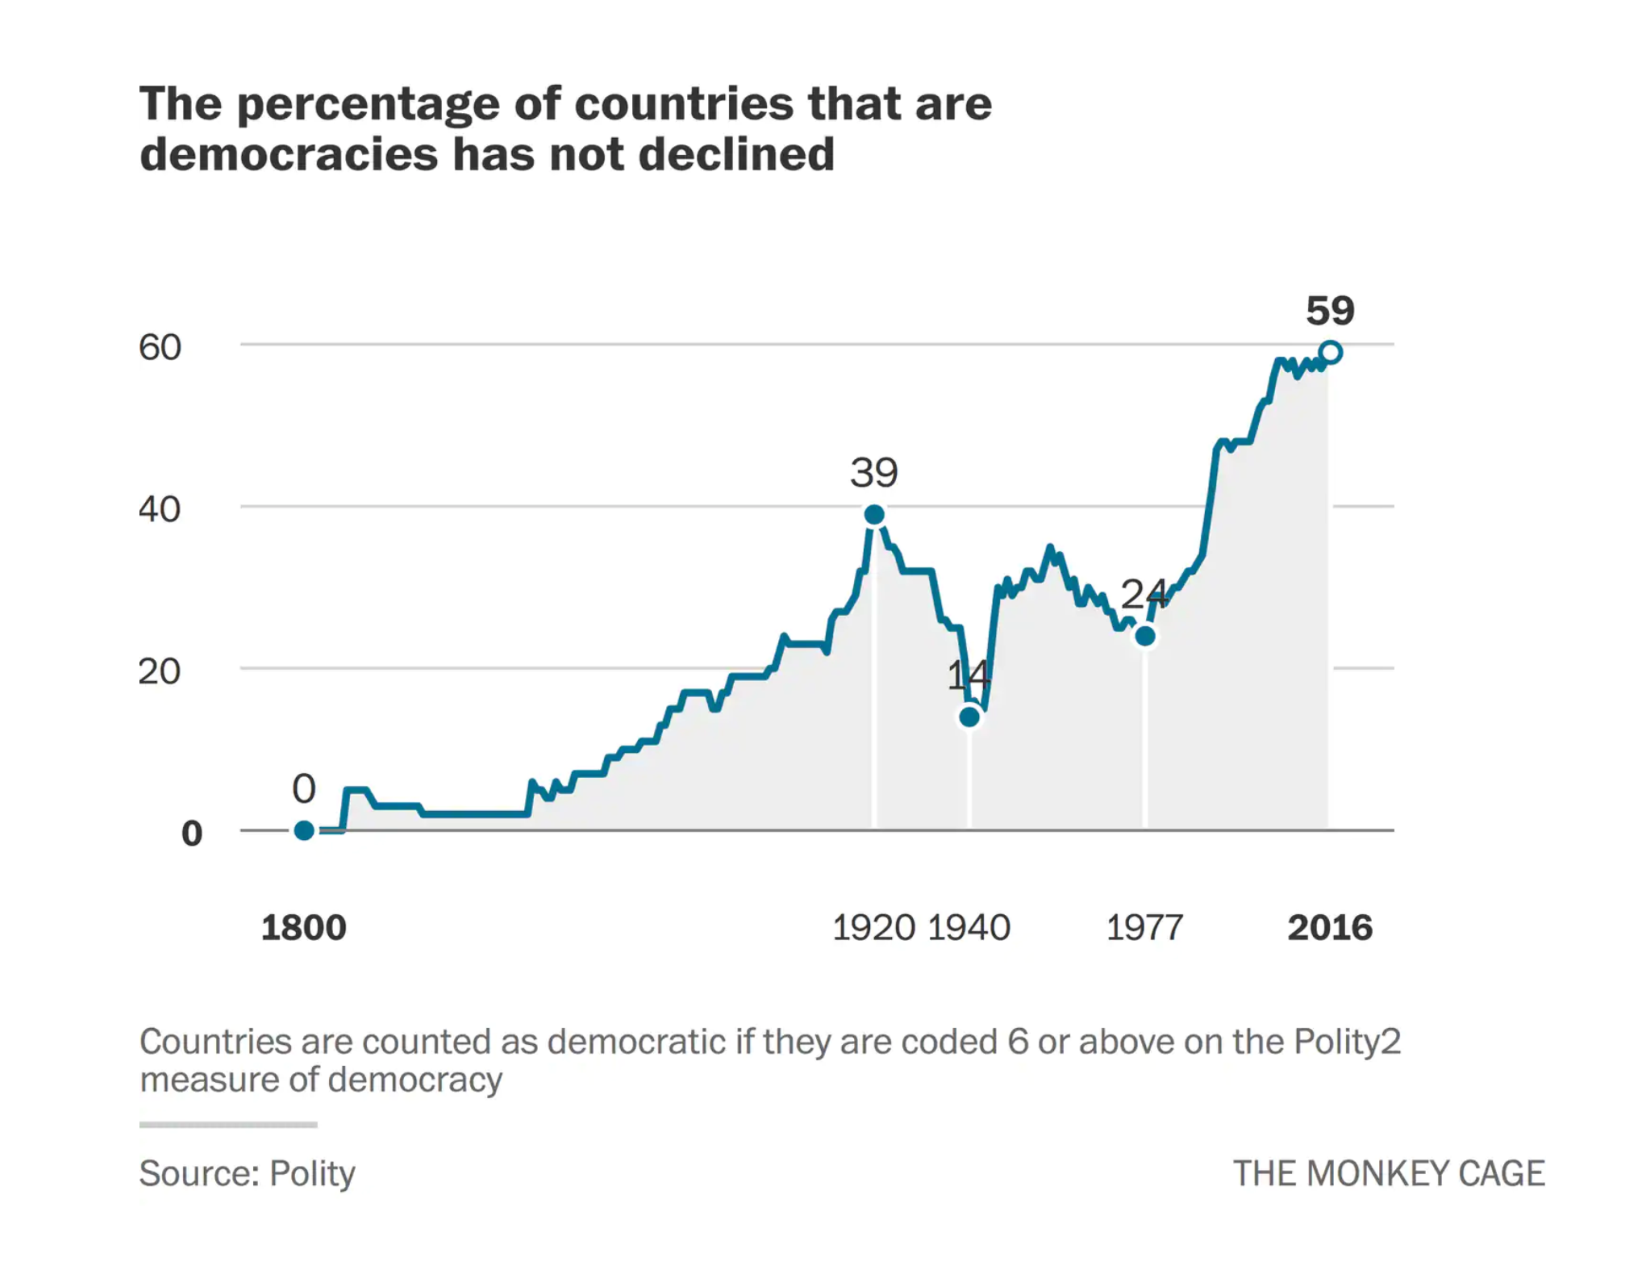
\includegraphics[scale=0.38]{Figs/dan}
	\end{figure}
\end{frame}

\begin{frame}{Definition and terminology}
How do we define an authoritarian regime?
	\pause
	\vspace{0.1cm}
	\begin{itemize}
		\item Cheibub, Gandhi, and Przeworski (2010)
		\item Geddes, Wright, and Frantz (2015)
	\end{itemize}
\end{frame}

\begin{frame}{Definition and terminology: Cheibub et al (2010)}
	\begin{columns}
    \column{0.55\linewidth}
	For a regime to be democratic, both the \textbf{chief executive office} and the \textbf{legislative body} must be filled by regular and competitive elections.
	\vspace{0.2cm}
	\begin{itemize}
	\item Ex ante uncertainty.
	\item Ex post irreversibility.
	\item Repeatability.
	\end{itemize}
    \column{0.42\linewidth}
    \centering
    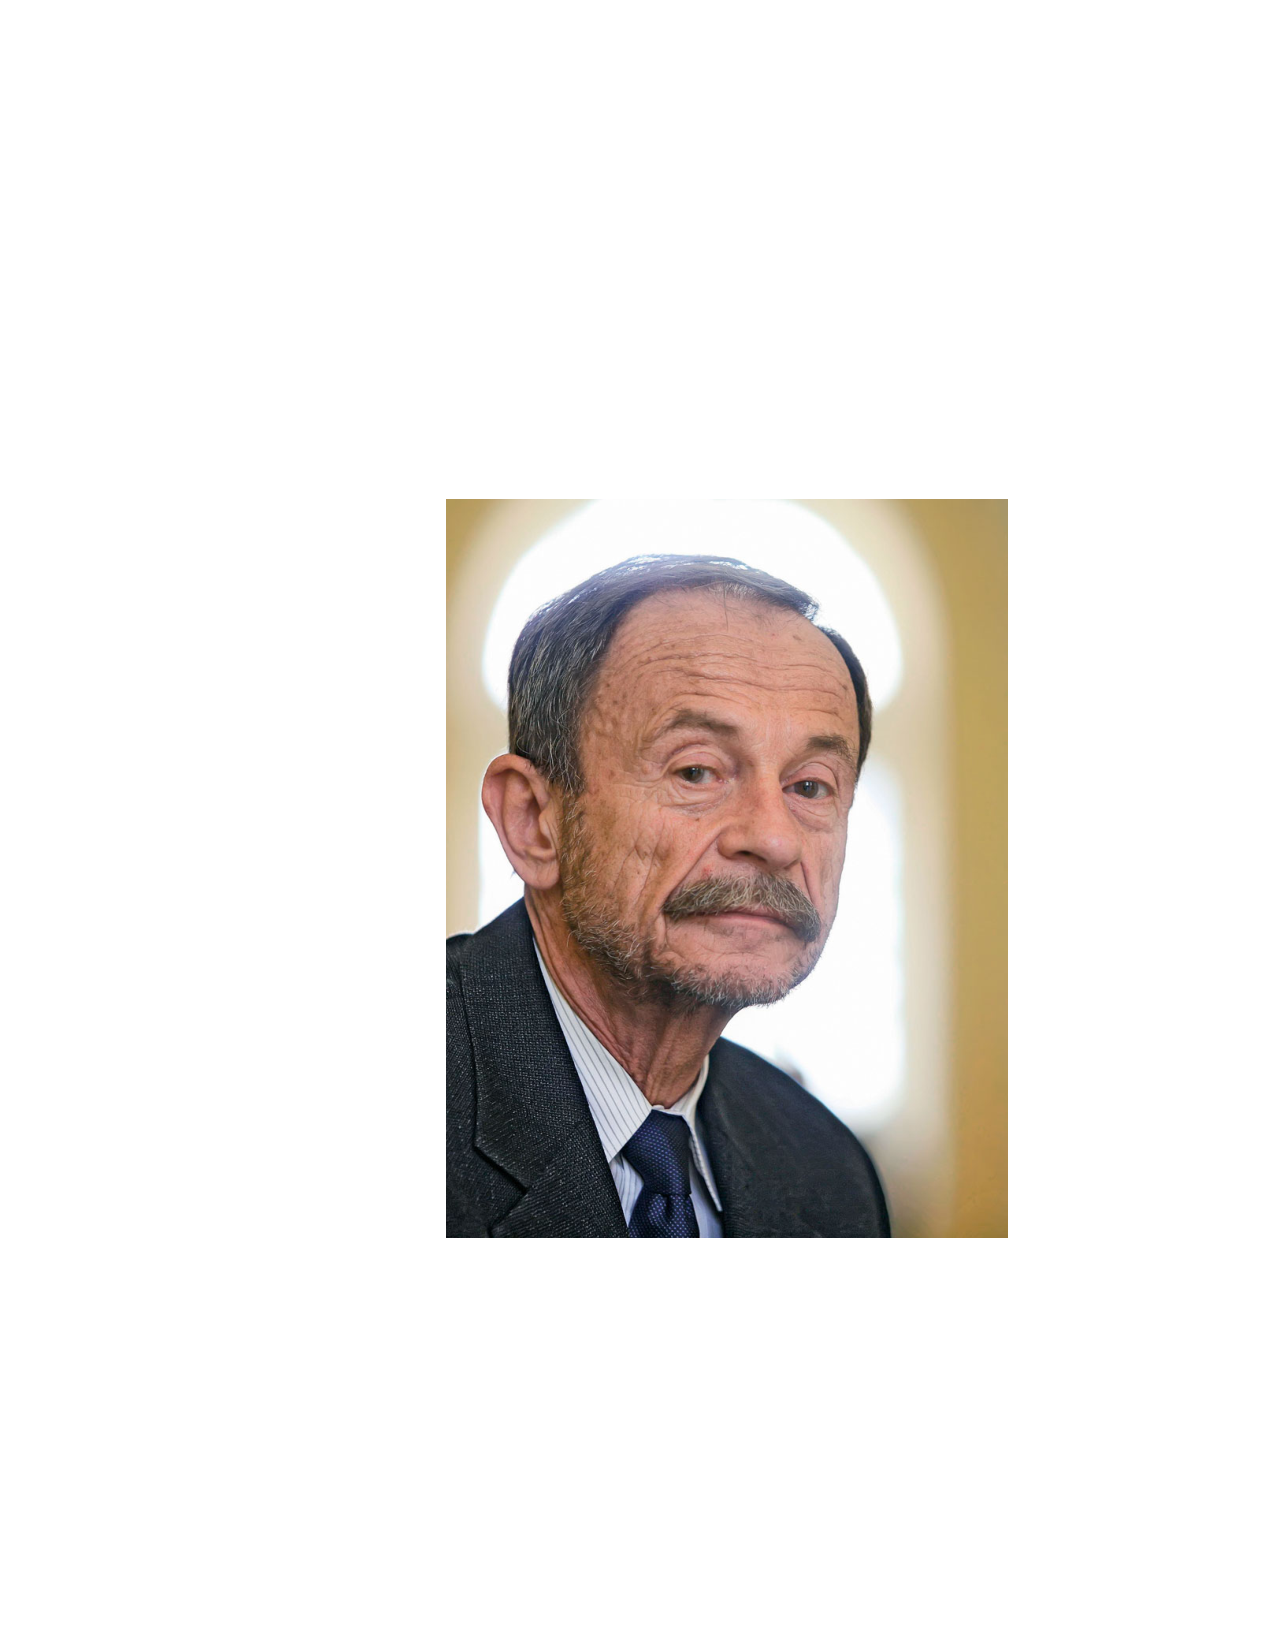
\includegraphics[scale=0.6]{Figs/as}
    \end{columns}
\end{frame}

\begin{frame}{Definition and terminology: Geddes et al (2015)}
	\begin{columns}
    \column{0.55\linewidth}
	\begin{itemize}
	\small
	\item An executive achieved power through undemocratic means. \textbf{``Undemocratic'' refers to any means besides direct, reasonably fair, competitive elections.}
	\vspace{0.1cm}
	\item The government achieved power through democratic means, but subsequently changed the formal or informal rules.
	\vspace{0.1cm}
	\item The military prevented parties that substantial numbers of citizens would be expected to vote for from competing and/or dictated important policy choices.
	\end{itemize}
    \column{0.42\linewidth}
    \centering
    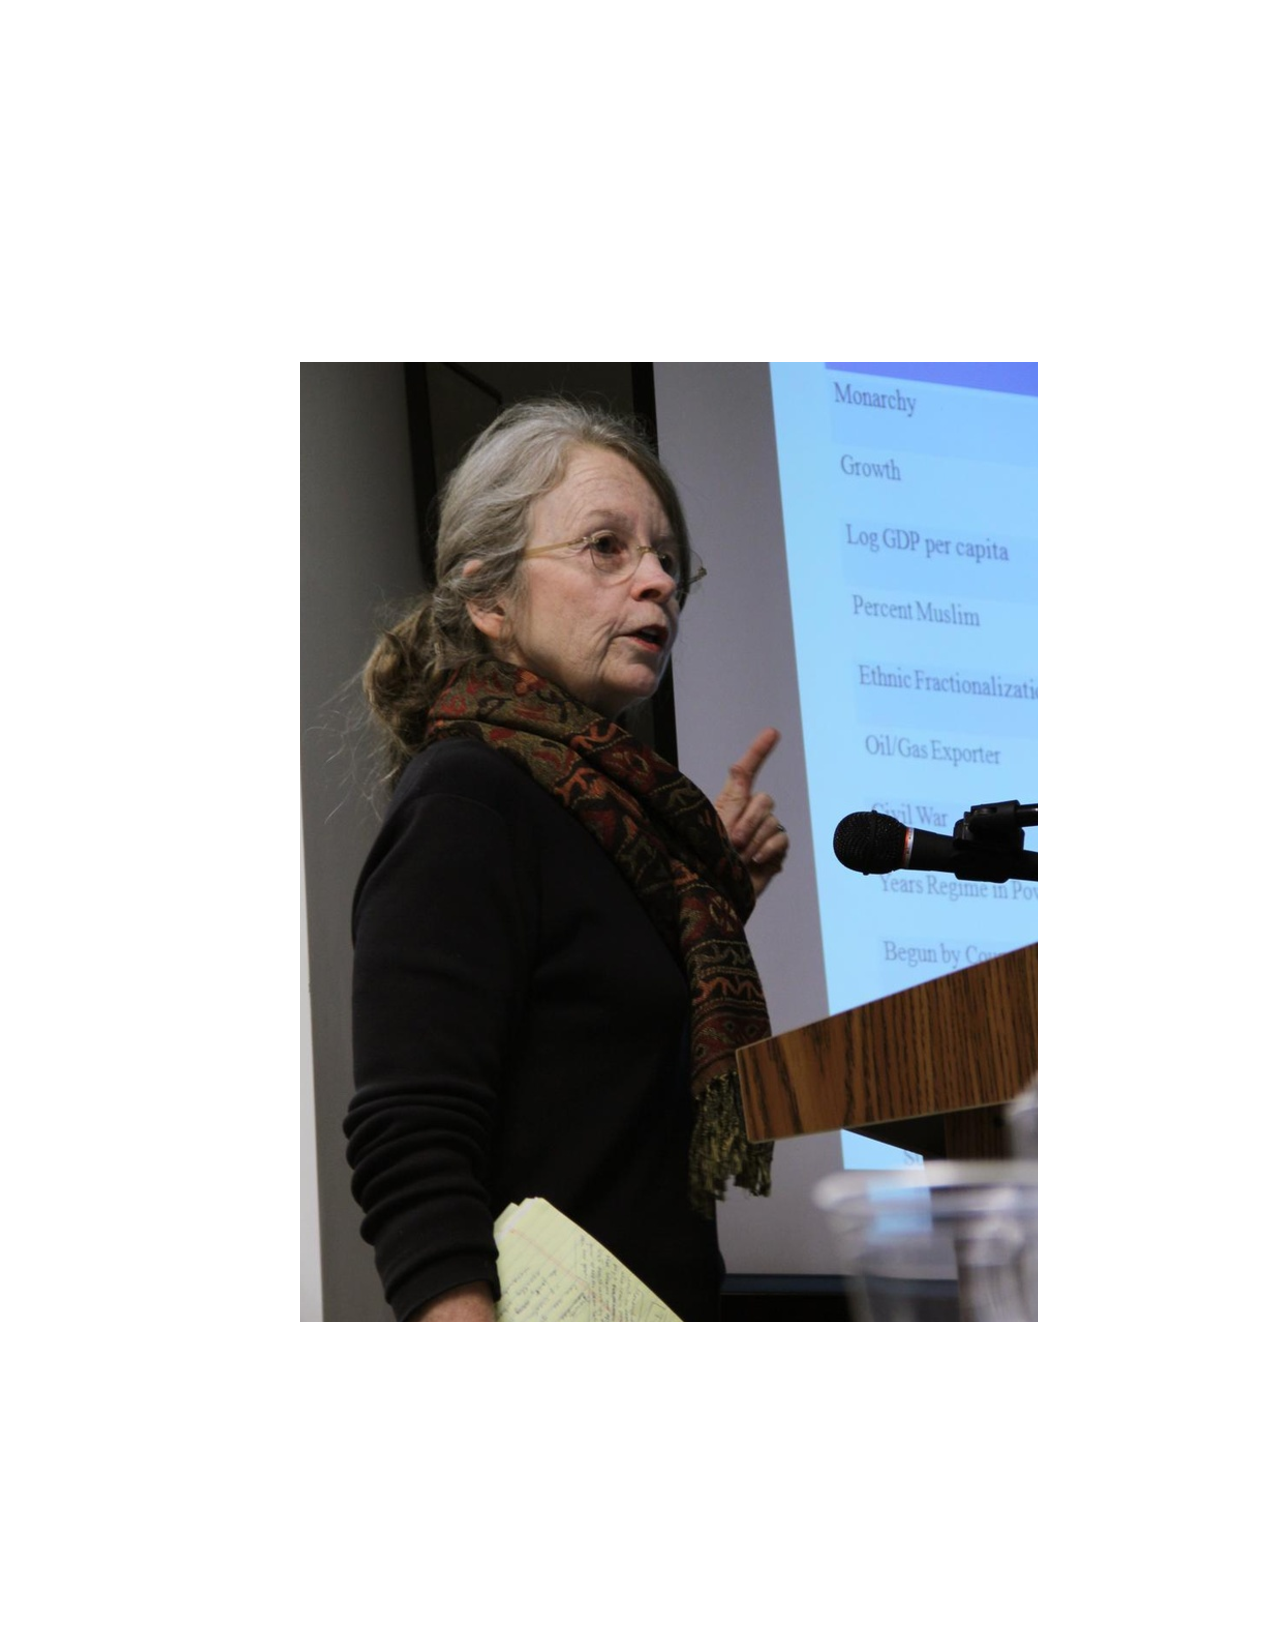
\includegraphics[scale=0.46]{Figs/bg}
    \end{columns}
\end{frame}

\begin{frame}{Definition and terminology}
	\begin{itemize}
	\item Autocracy vs. dictatorship.
	\item Totalitarianism vs. authoritarianism.
	\end{itemize}
\end{frame}

\begin{frame}{Authoritarian regimes in the world}
	\begin{itemize}
		\item Democracy and Dictatorship Database (Cheibub et al)
		\item Autocratic Regime Data (Geddes et al)
	\end{itemize}
\end{frame}

\begin{frame}{Authoritarian regimes in the world}
	\begin{figure}
	\centering
	\subfigure{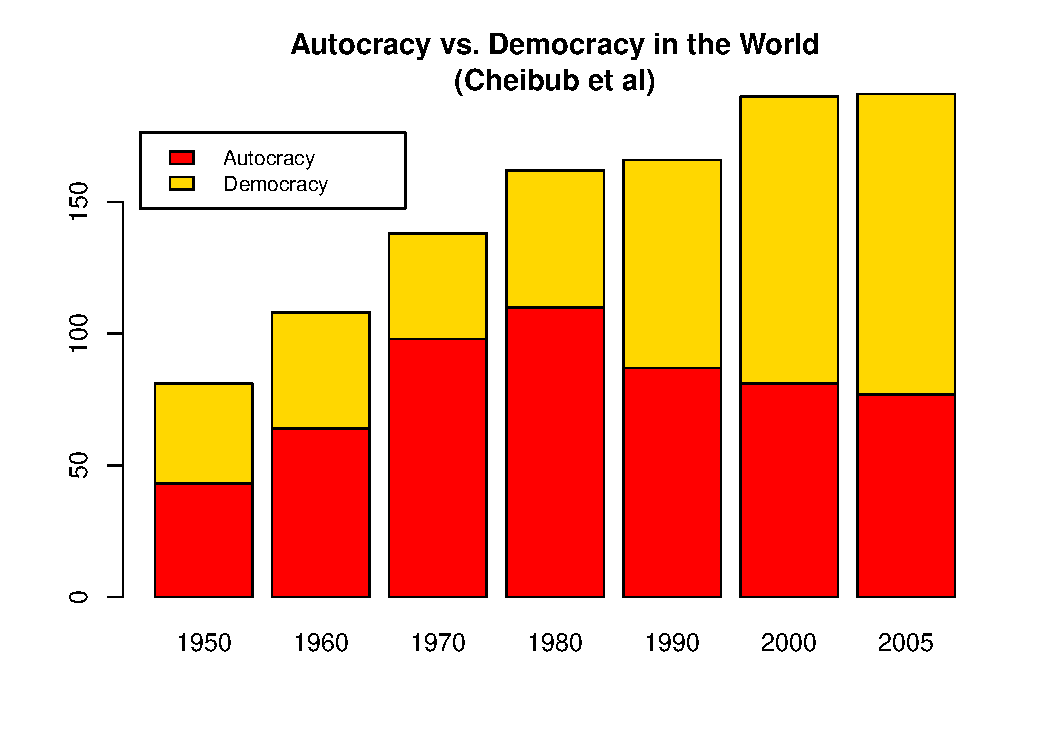
\includegraphics[scale=0.3]{Figs/dd_cpg}}
	\subfigure{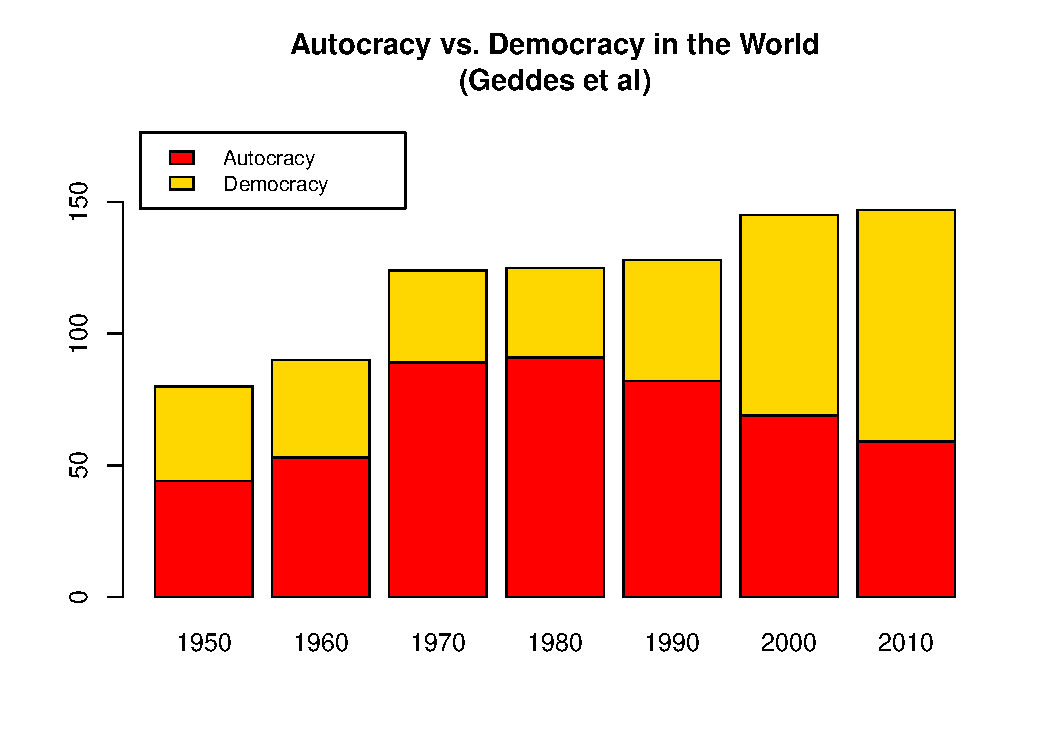
\includegraphics[scale=0.3]{Figs/dd_gwf}}	
	\end{figure}
\end{frame}

\begin{frame}{Authoritarian regimes in the world}
	\begin{figure}
	\centering
	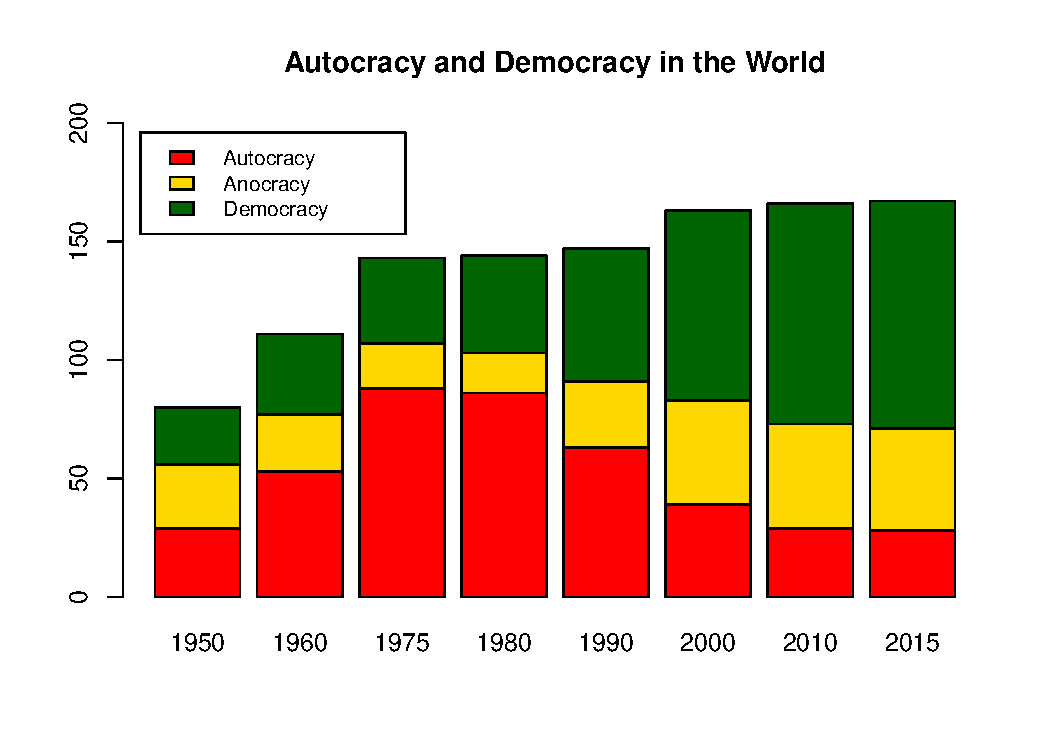
\includegraphics[scale=0.6]{Figs/Polity/pl_history}
	\end{figure}
\end{frame}

\begin{frame}{Varieties of authoritarian regimes}
	\begin{itemize}
		\item Who controls the ruling power?
		\item Who has influences over policy making?
	\end{itemize}
\end{frame}

\begin{frame}{Varieties of authoritarian regimes}
	\begin{itemize}
		\item Military
		\item Single-party
		\item Personalist
		\item Monarchy
	\end{itemize}
\end{frame}

\begin{frame}{Varieties of authoritarian regimes}
	\begin{figure}
	\centering
	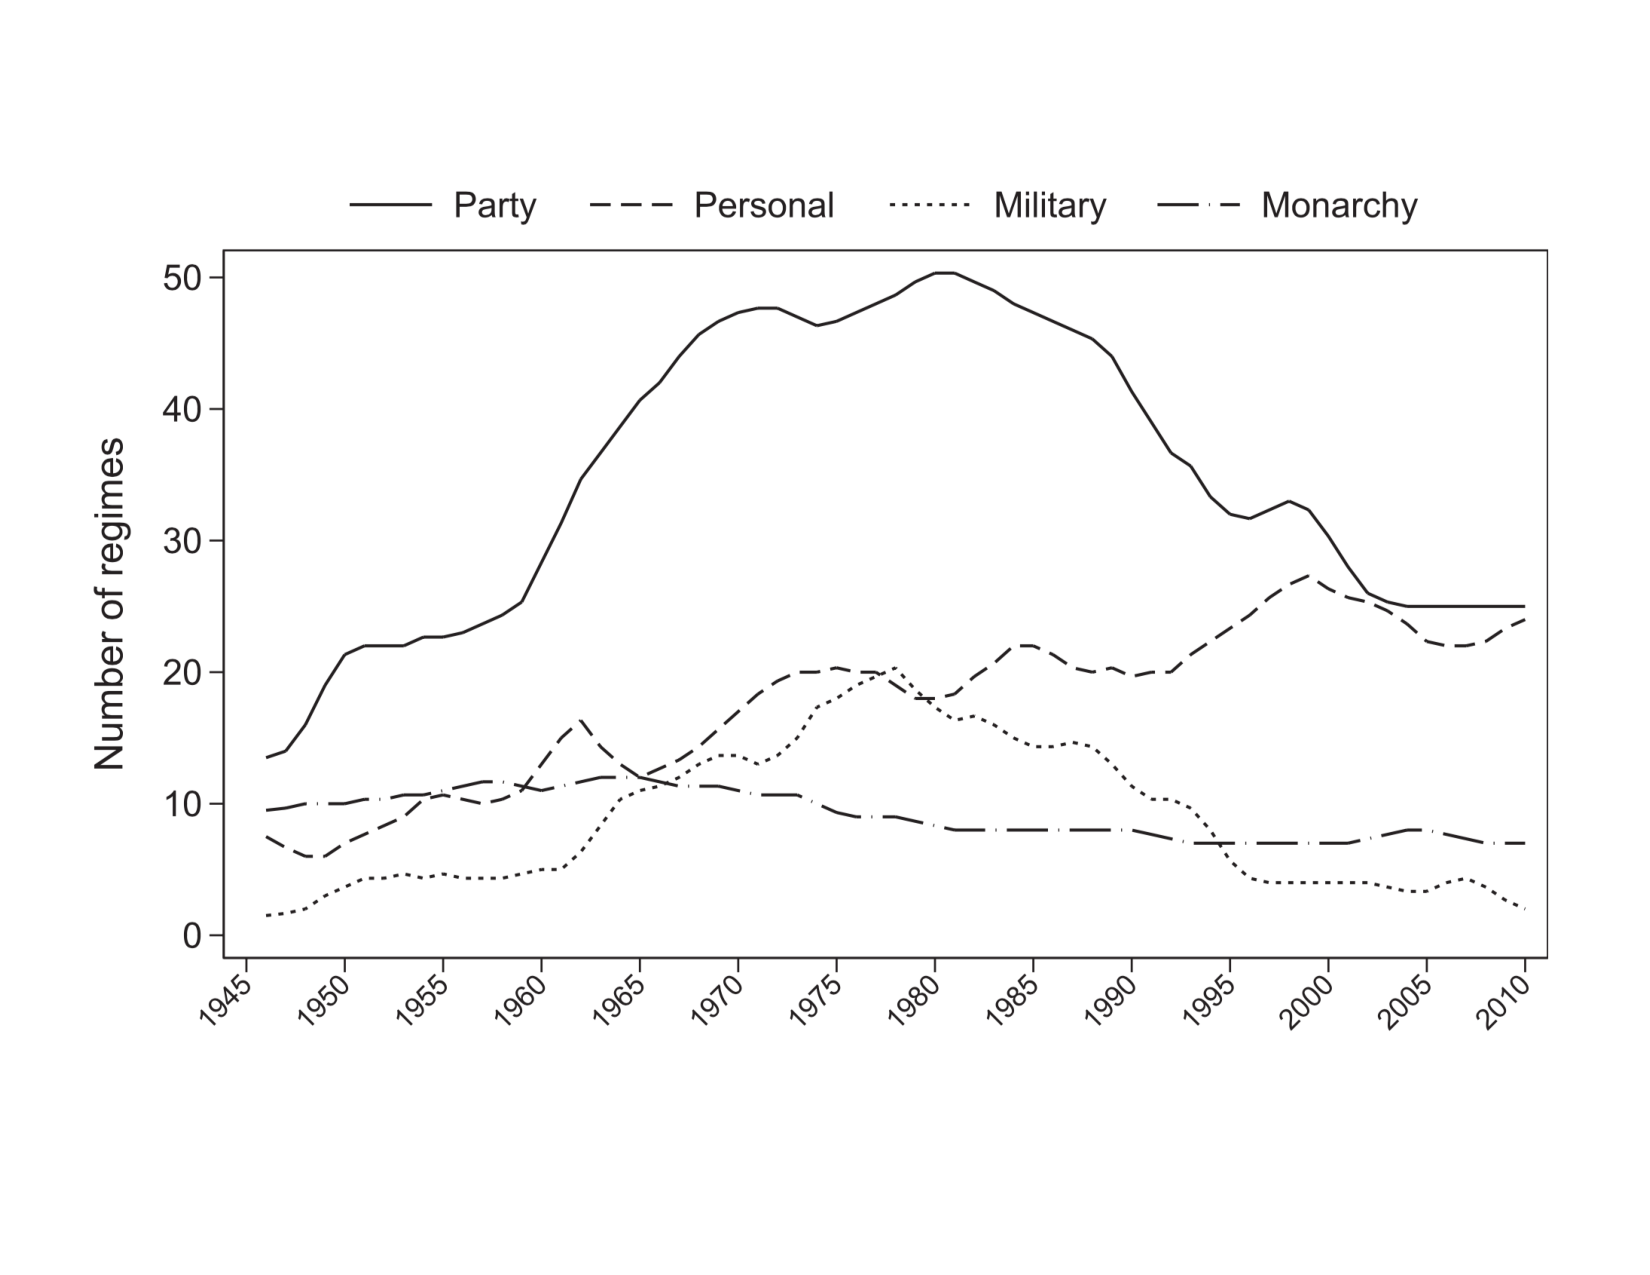
\includegraphics[scale=0.4]{Figs/GWF/type}
	\end{figure}
\end{frame}

\begin{frame}{Varieties of authoritarian regimes: Military regime}
	\begin{figure}
	\centering
	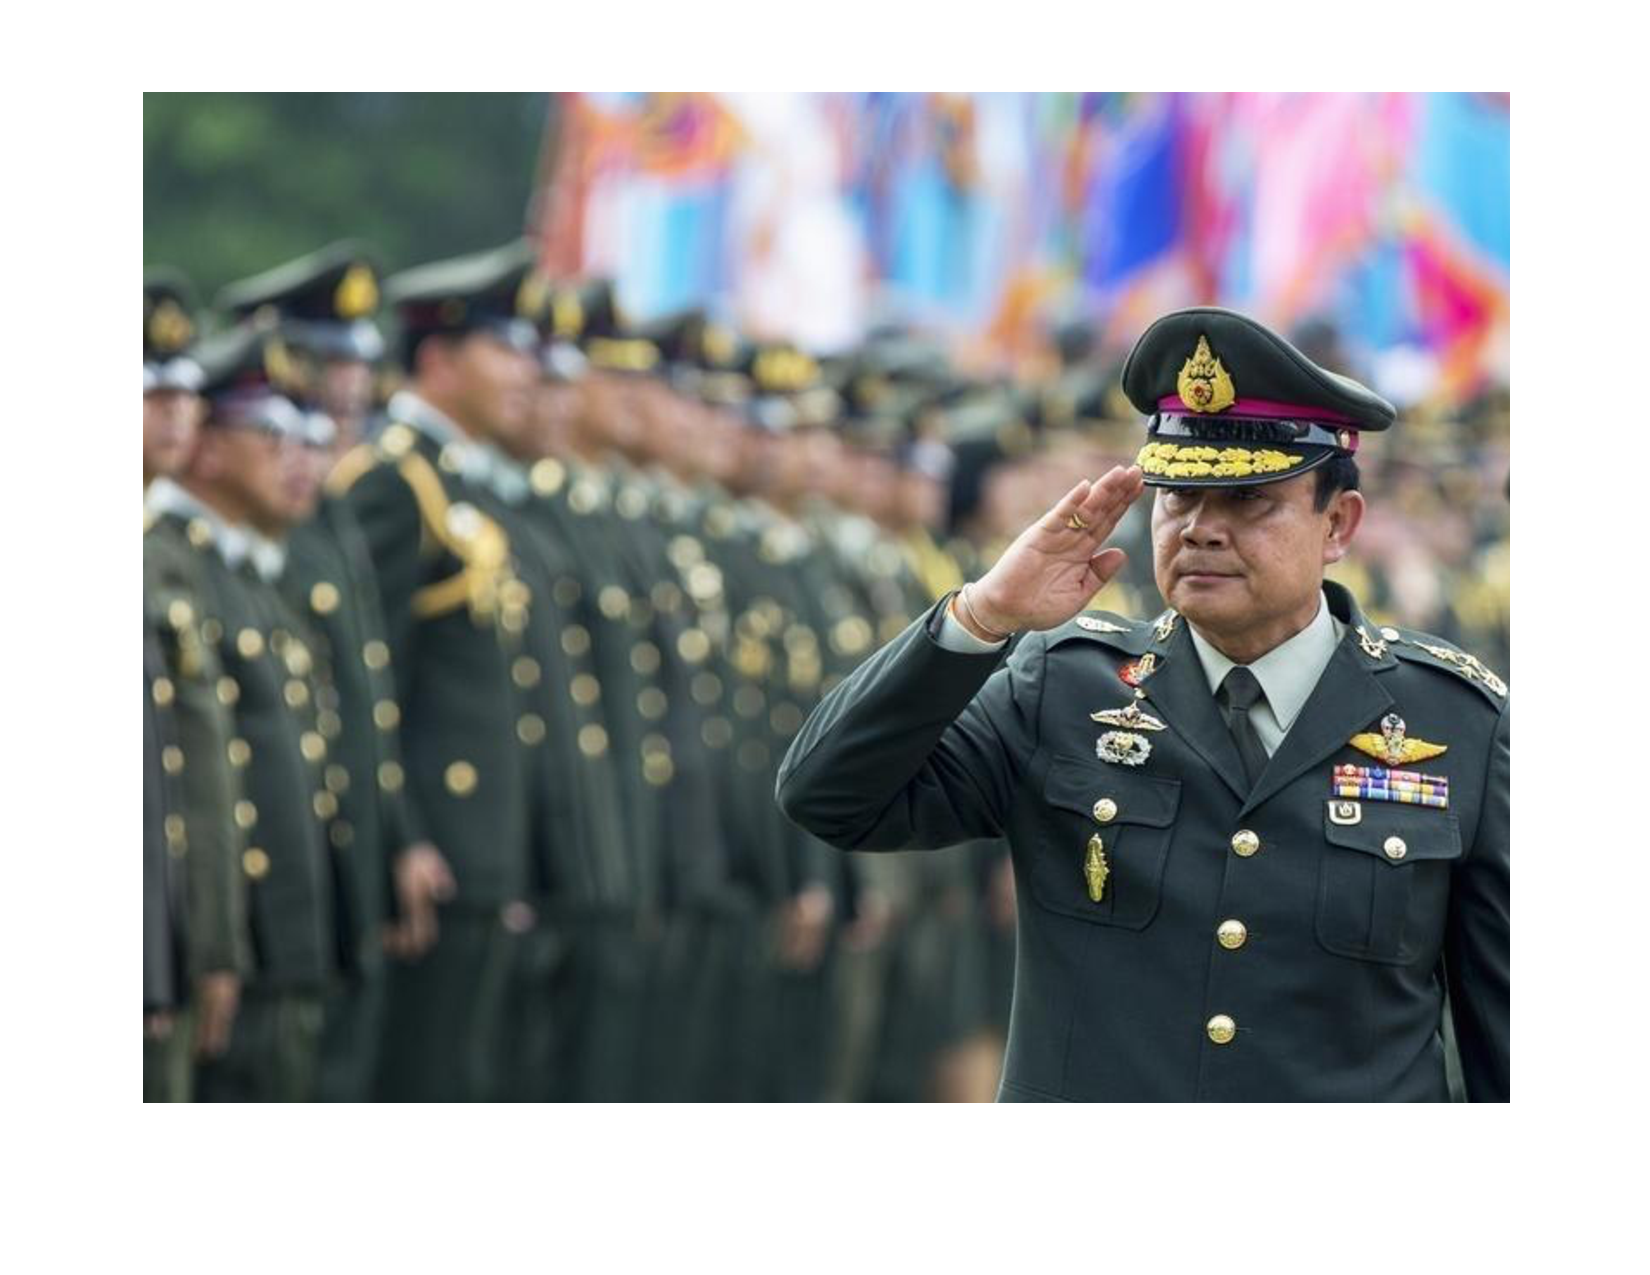
\includegraphics[scale=0.3]{Figs/Countries/thailand}
	\end{figure}
	\pause
	\centering
	Prayut Chan-o-cha, the Prime Minister of Thailand (2014-), and the Thai junta.
\end{frame}

\begin{frame}{Varieties of authoritarian regimes: Single-party regime}
	\begin{figure}
	\centering
	\includegraphics[scale=0.34]{Figs/Countries/china2}
	\end{figure}
	\centering
	Xi Jiping, the General Secretary of the Chinese Communist Party (2013-), along with the Politburo Standing Committee.
\end{frame}

\begin{frame}{Varieties of authoritarian regimes: Personalist regime}
	\begin{columns}
    \column{0.6\linewidth}
	\begin{itemize}
	\small
	\item 1937: Born to a peasant family in a desert village near Tikrit, north of Baghdad.
	\item 1968: Baathists worked with army officers to overthrow the Arif regime. Ahmad Hasan al-Bakr (Saddam's cousin) became president.
	\item 1979: Took over as the President.
	\item 1980-1988: Iran-Iraq war resulted in stalemate.
	\item 1990-1991: Iraq invaded Kuwait.
	\item 2003: US-Iraq war began.
	\item 2006: Executed for crimes against humanity.  
	\end{itemize}
    \column{0.4\linewidth}
    \centering
    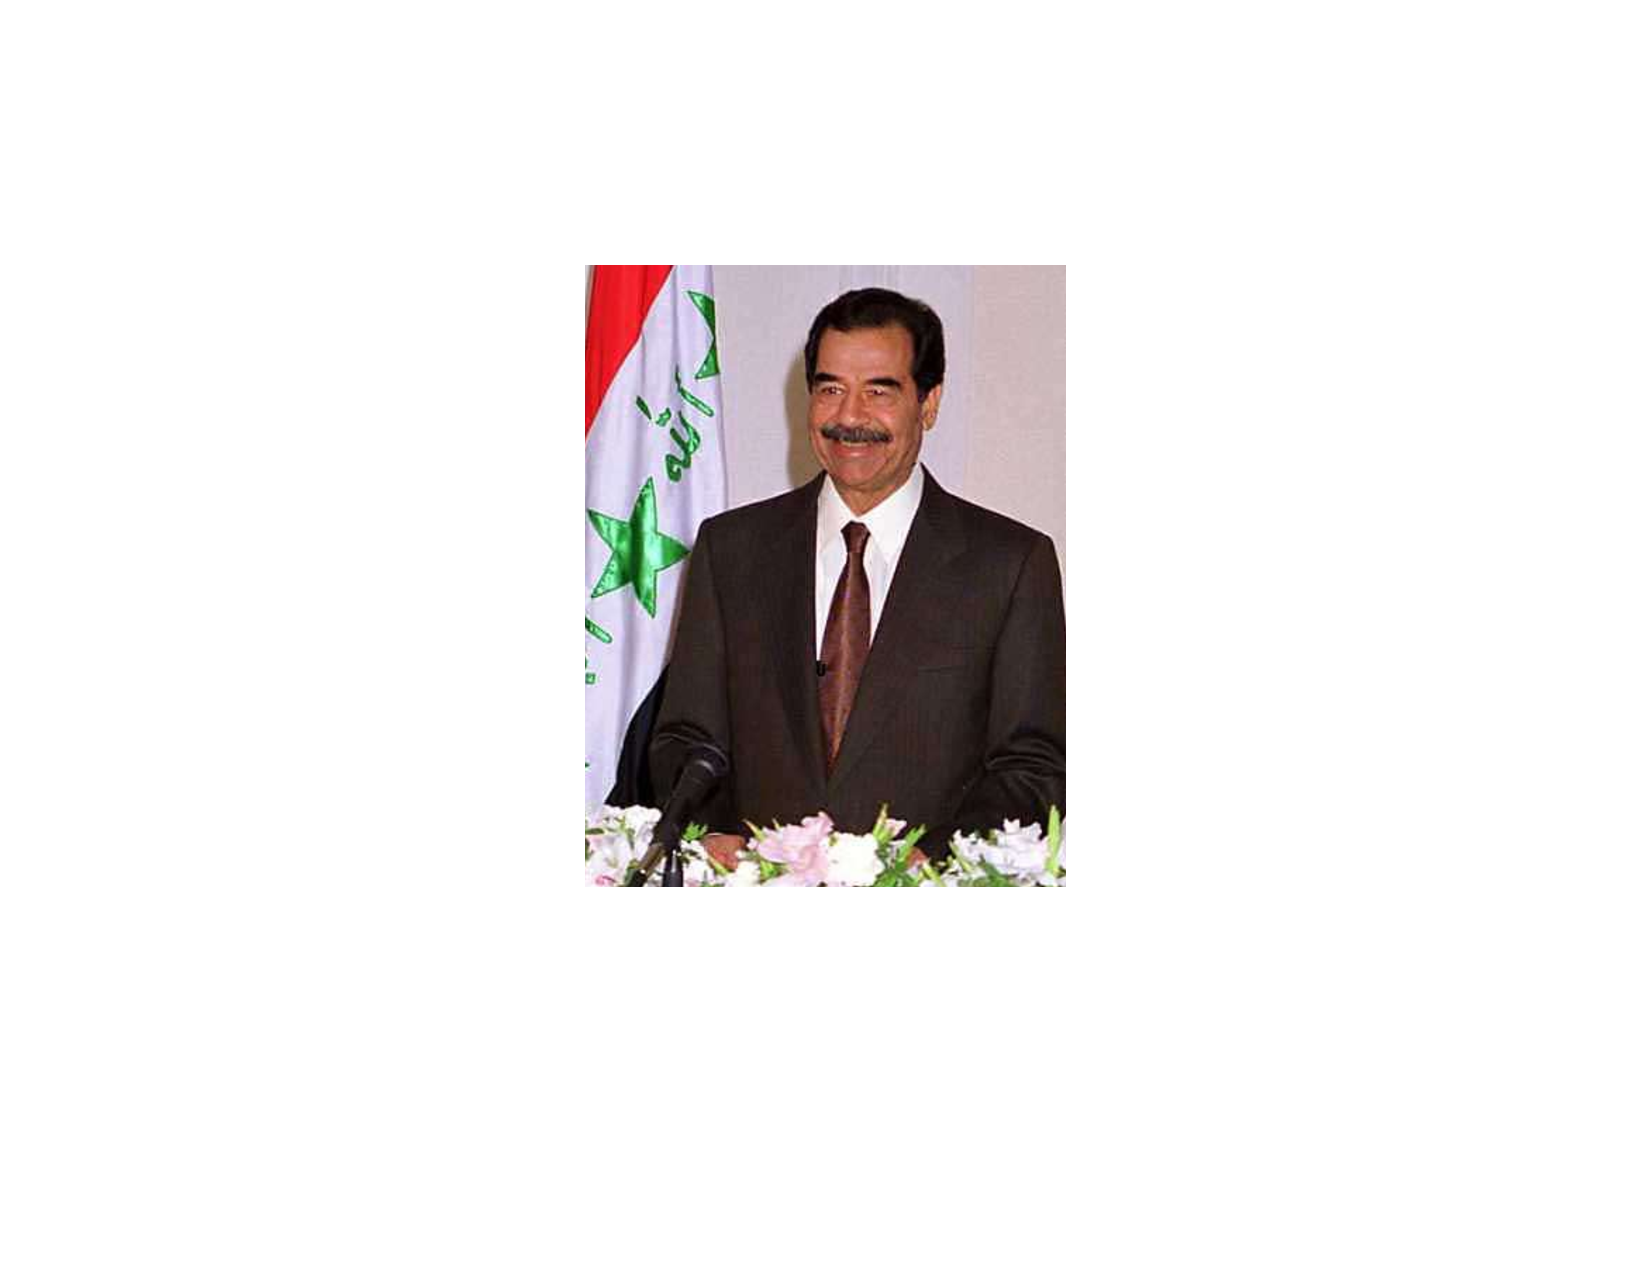
\includegraphics[scale=0.7]{Figs/Countries/iraq}
    \end{columns}
\end{frame}

\begin{frame}{Varieties of authoritarian regimes: Monarchy}
	\begin{figure}
	\centering
    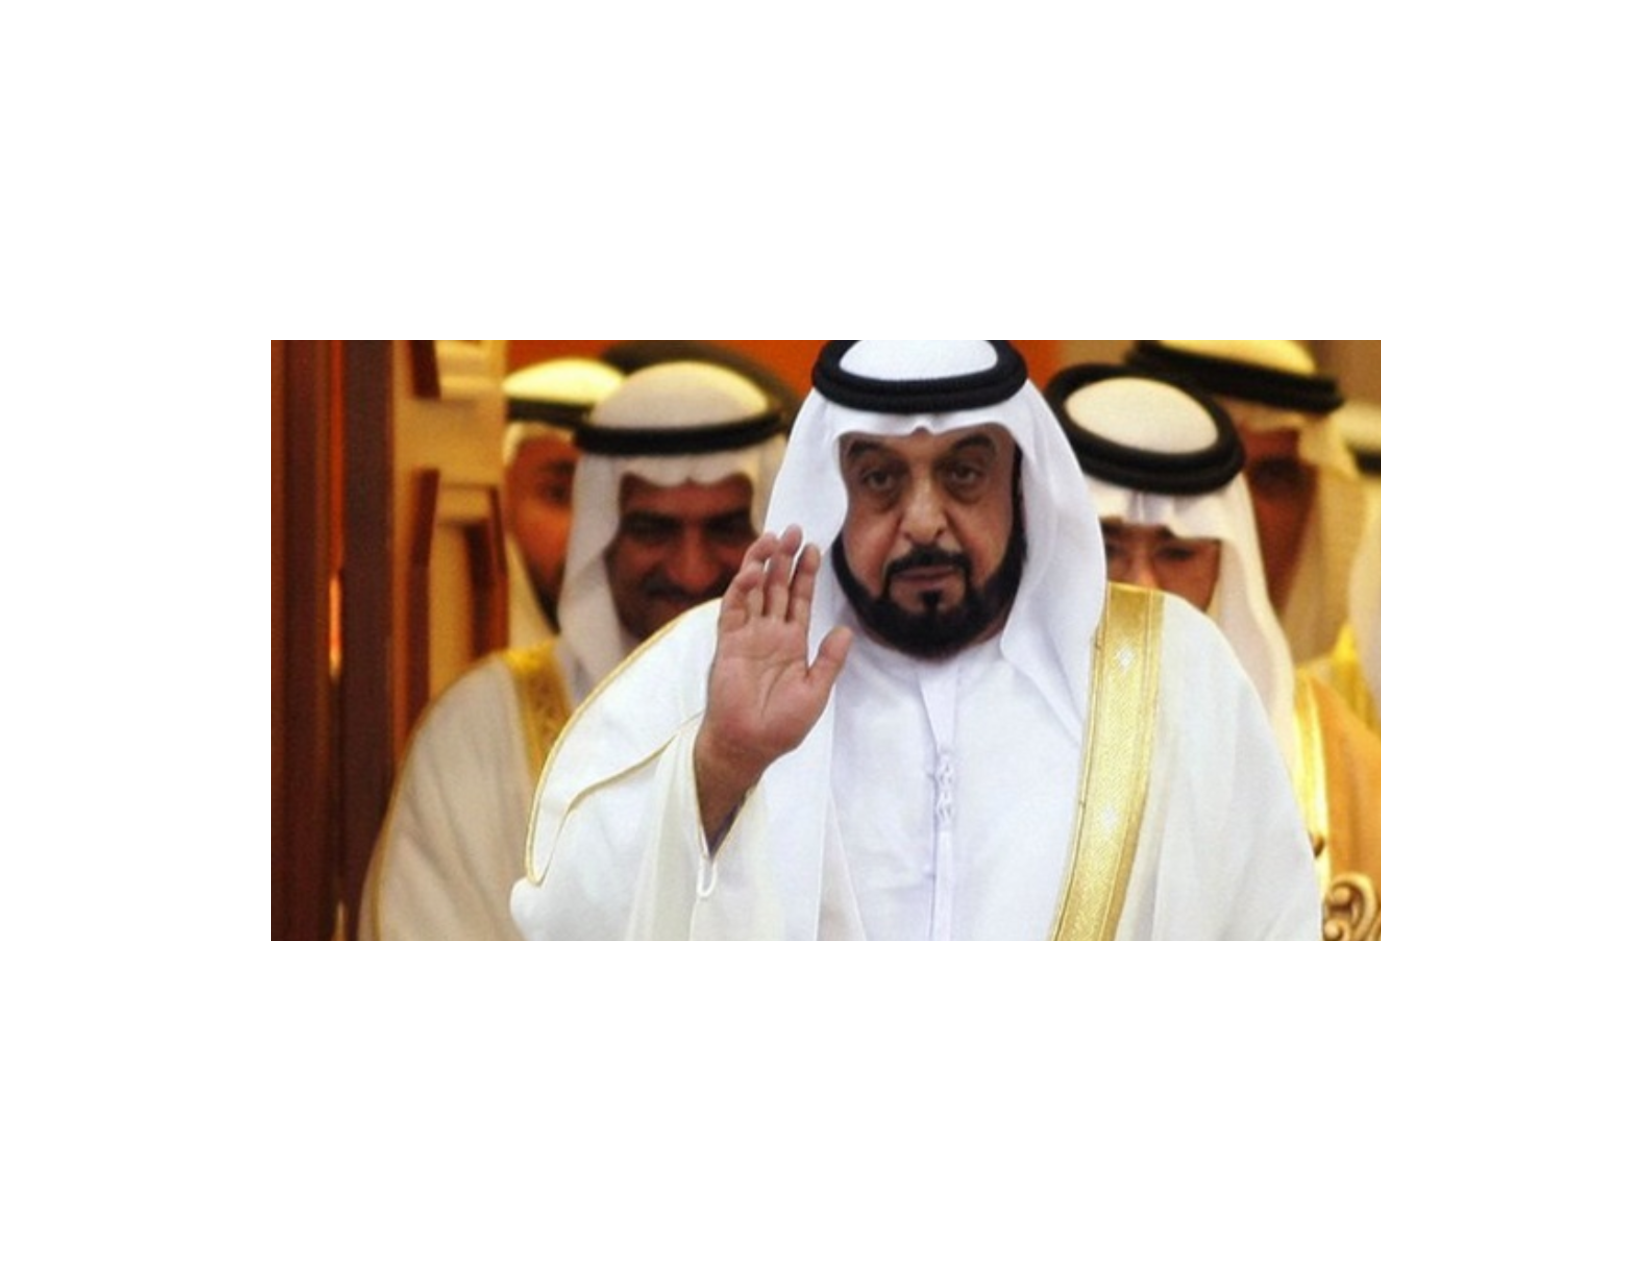
\includegraphics[scale=0.32]{Figs/Countries/uae}
	\end{figure}
	\pause
	\begin{itemize}
	\small
	\item A federation of seven constituent emirates/monarchies, who form the Federal Supreme Council.
	\item The President and the Vice President elected by the Federal Supreme Council.
	\item The Presidency (head of state) hereditary to the Al Nahyan clan of Abu Dhabi.
	\item The Vice-Presidency (head of government) hereditary to the Al Maktoum clan of Dubai.
	\end{itemize}
\end{frame}

\begin{frame}
What are the pros and cons of a typology of authoritarian regimes?
\end{frame}

\begin{frame}{Hybrid regime}
	\begin{figure}
	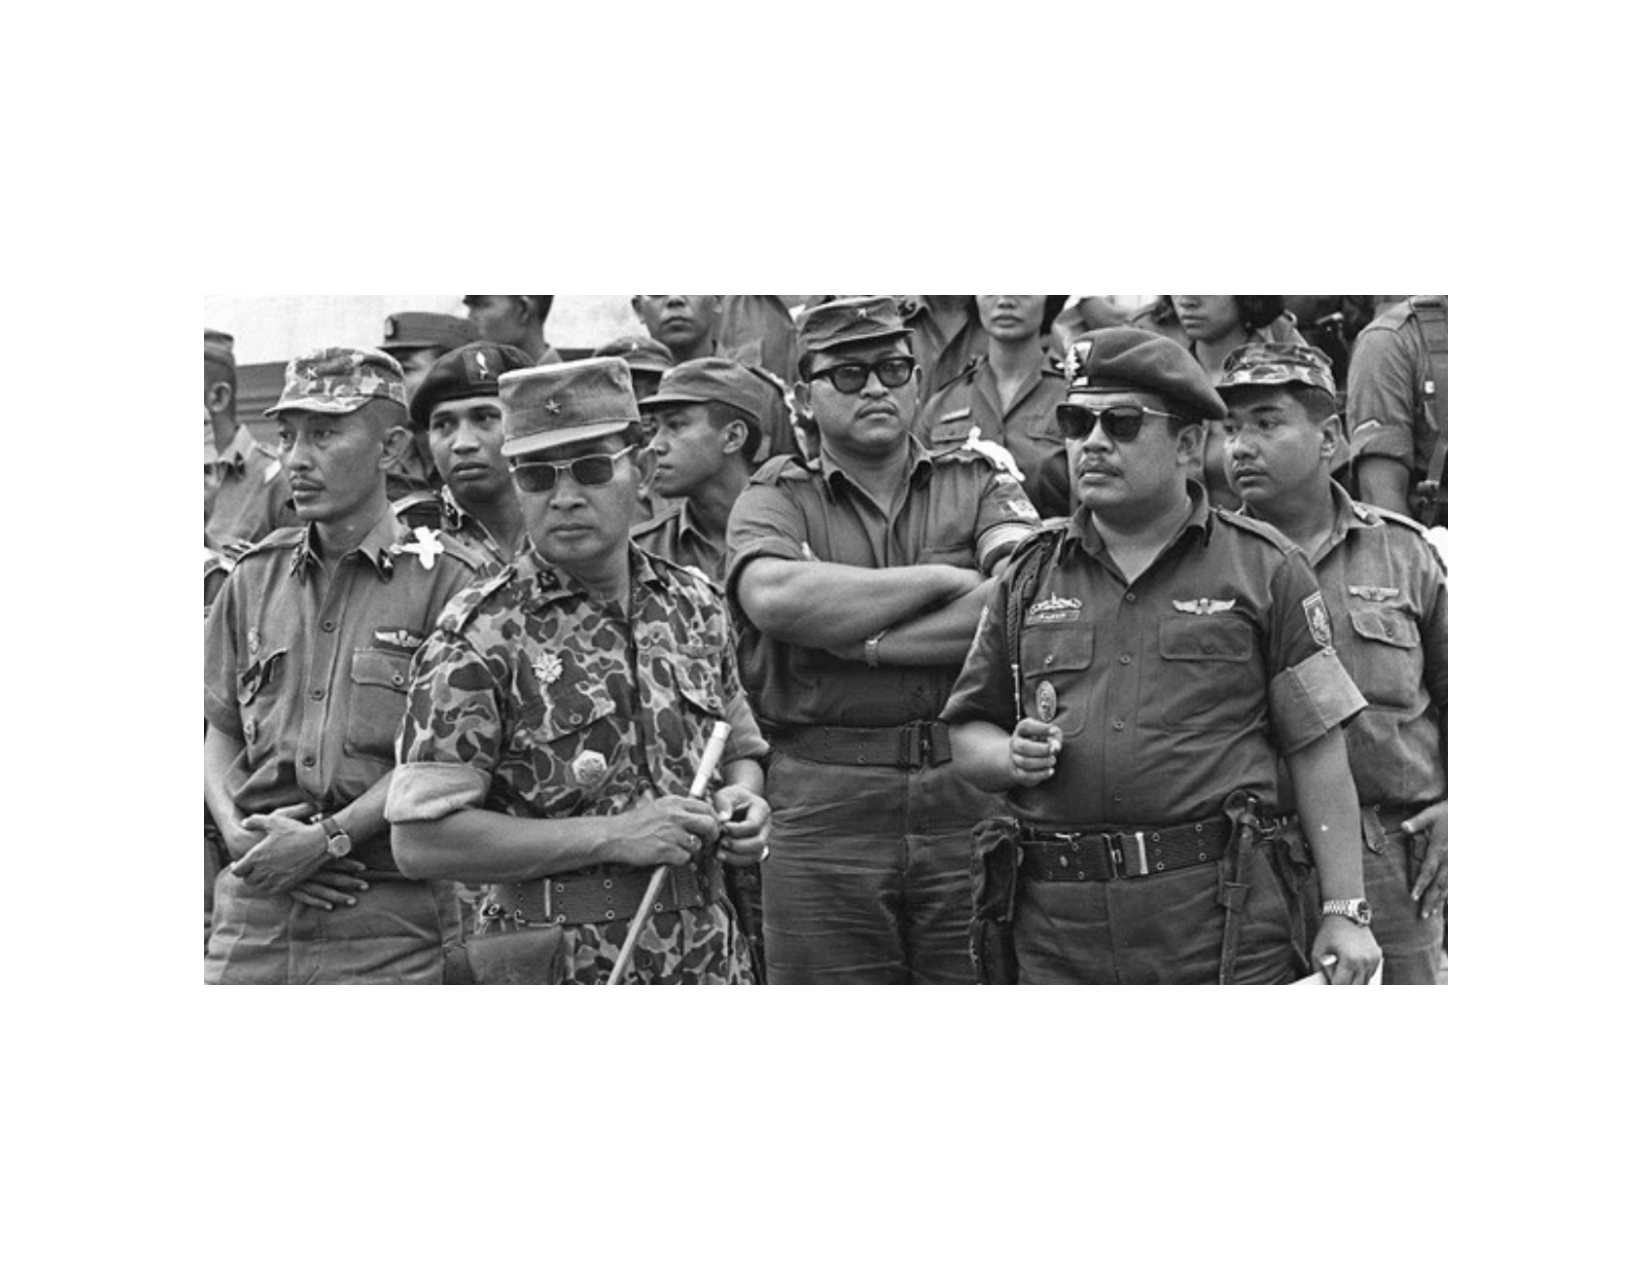
\includegraphics[scale=0.35]{Figs/Countries/indonesia}
	\end{figure}
	\pause
	\small
	New Order in Indonesia (1966-1998) \\
	\pause $\quad =$ Personalist leader (Gen. Suharto) $+$ military junta $+$ mass political party (Golkar).
\end{frame}

\begin{frame}{Hybrid regime}
	\begin{figure}
	\centering
	\subfigure{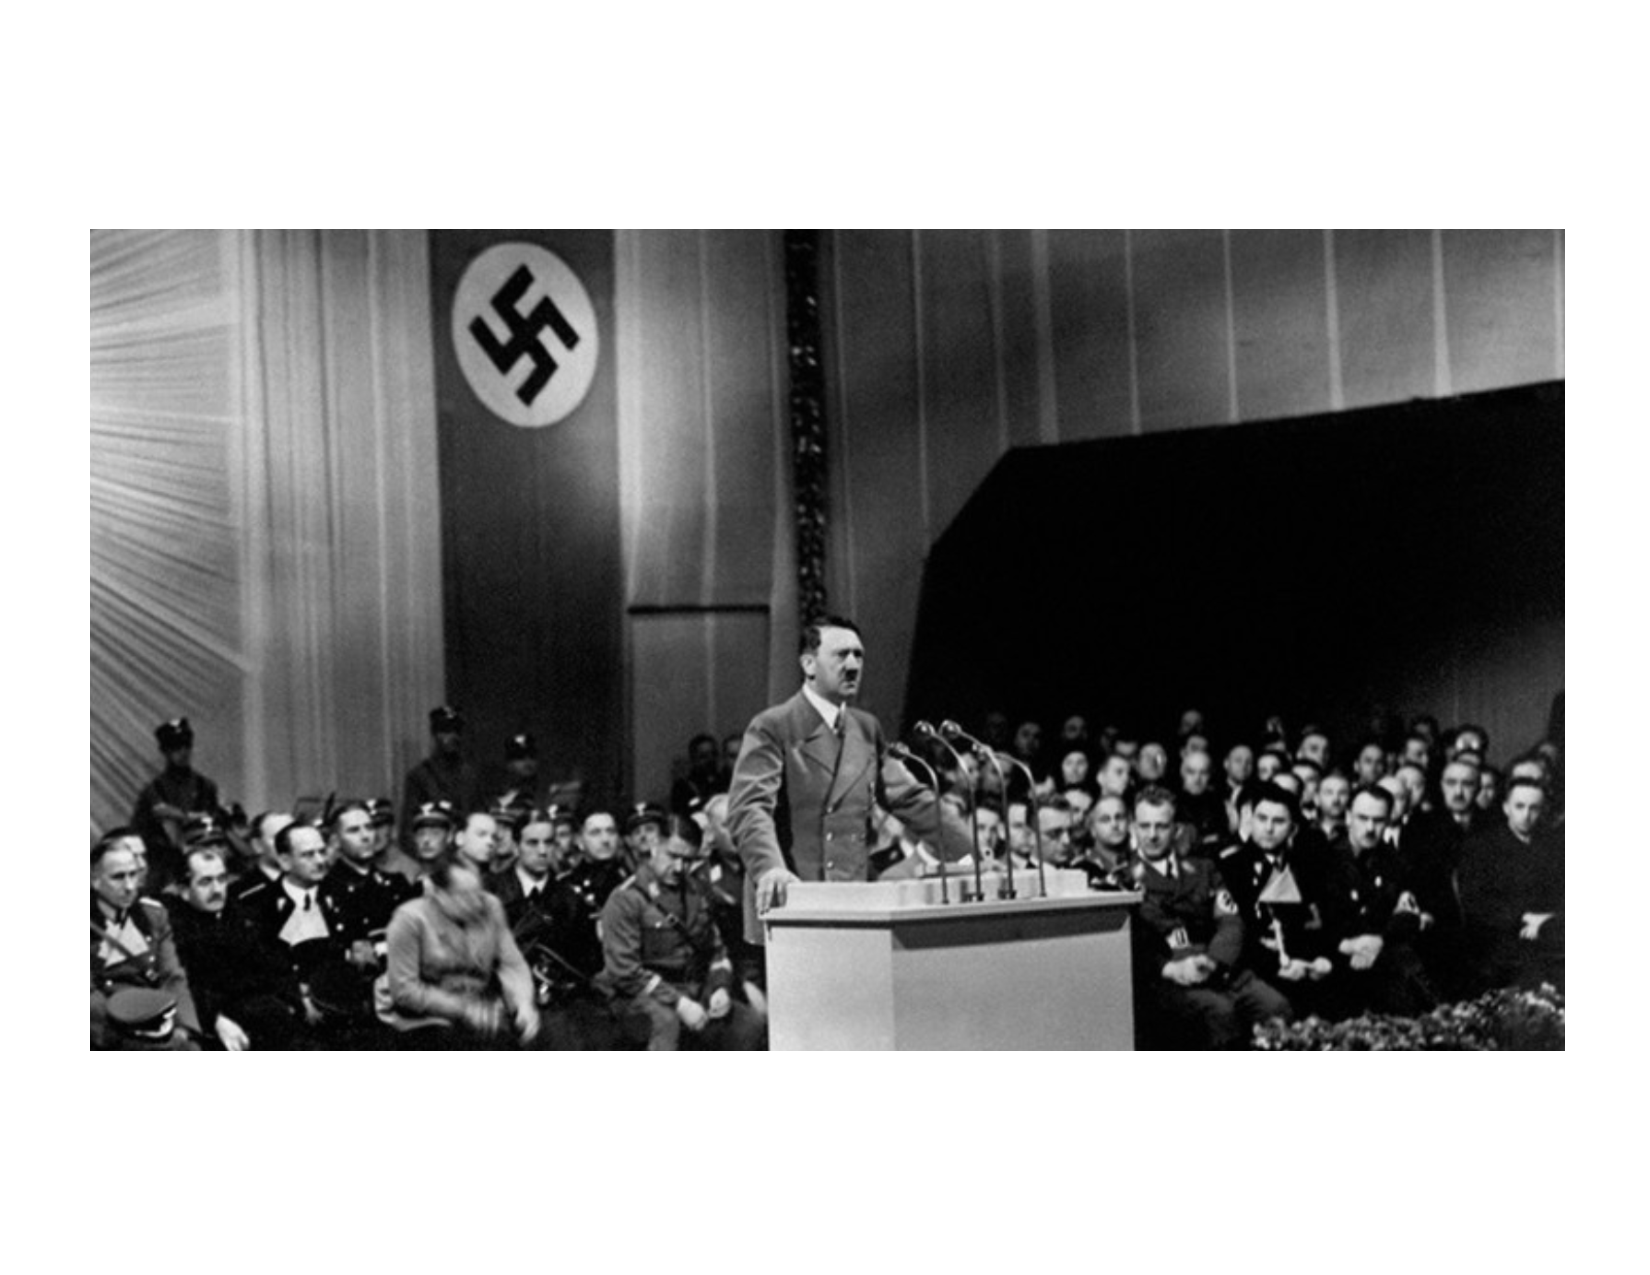
\includegraphics[scale=0.21]{Figs/Countries/nazi}}	
	\hspace{0.1cm}
	\subfigure{\includegraphics[scale=0.2]{Figs/Countries/northkorea}}
	\end{figure}
	Are they the combination of?
\end{frame}

\begin{frame}{Varieties of authoritarian regimes: Alternatives}
	\begin{figure}
	\centering
	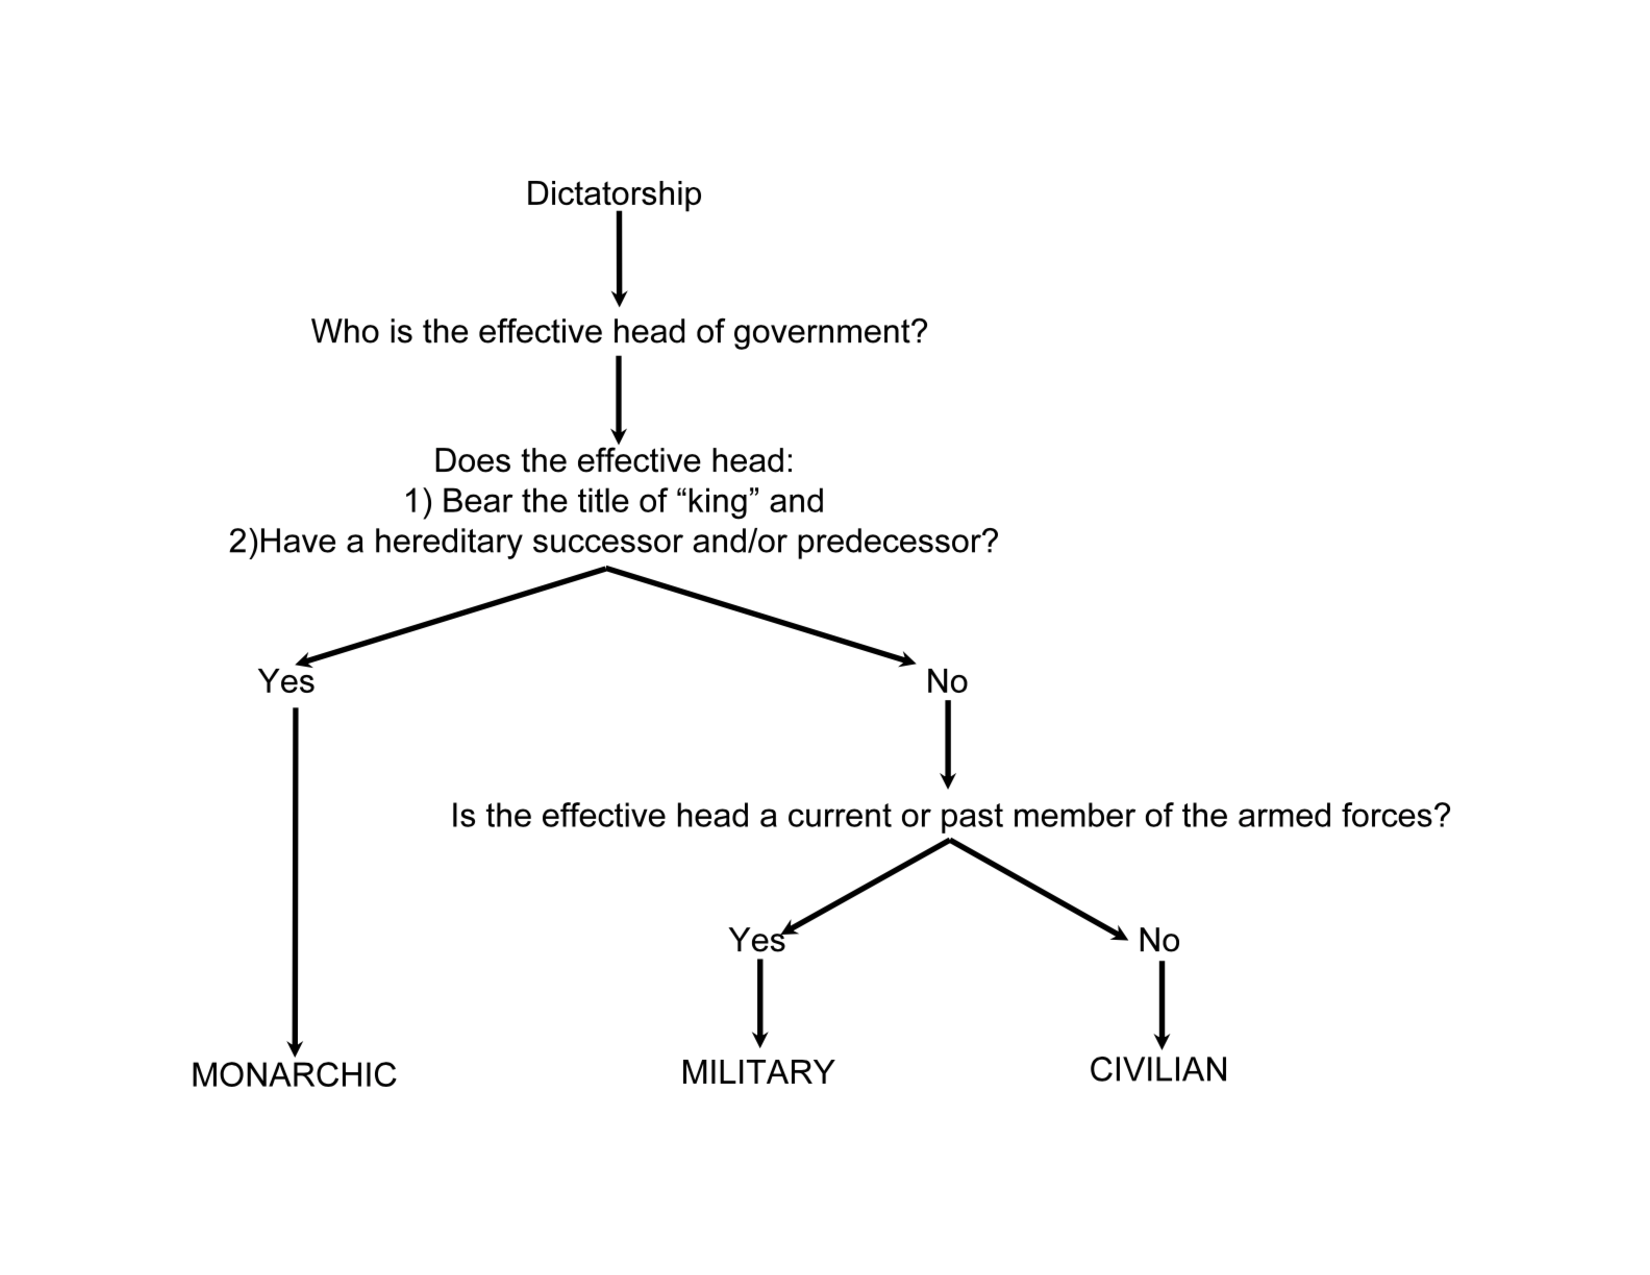
\includegraphics[scale=0.45]{Figs/cpg}
	\end{figure}
\end{frame}

\begin{frame}
Do different types of authoritarian regimes matter?
\end{frame}

\begin{frame}{Regime types and authoritarian survival}
	\begin{figure}
	\centering
	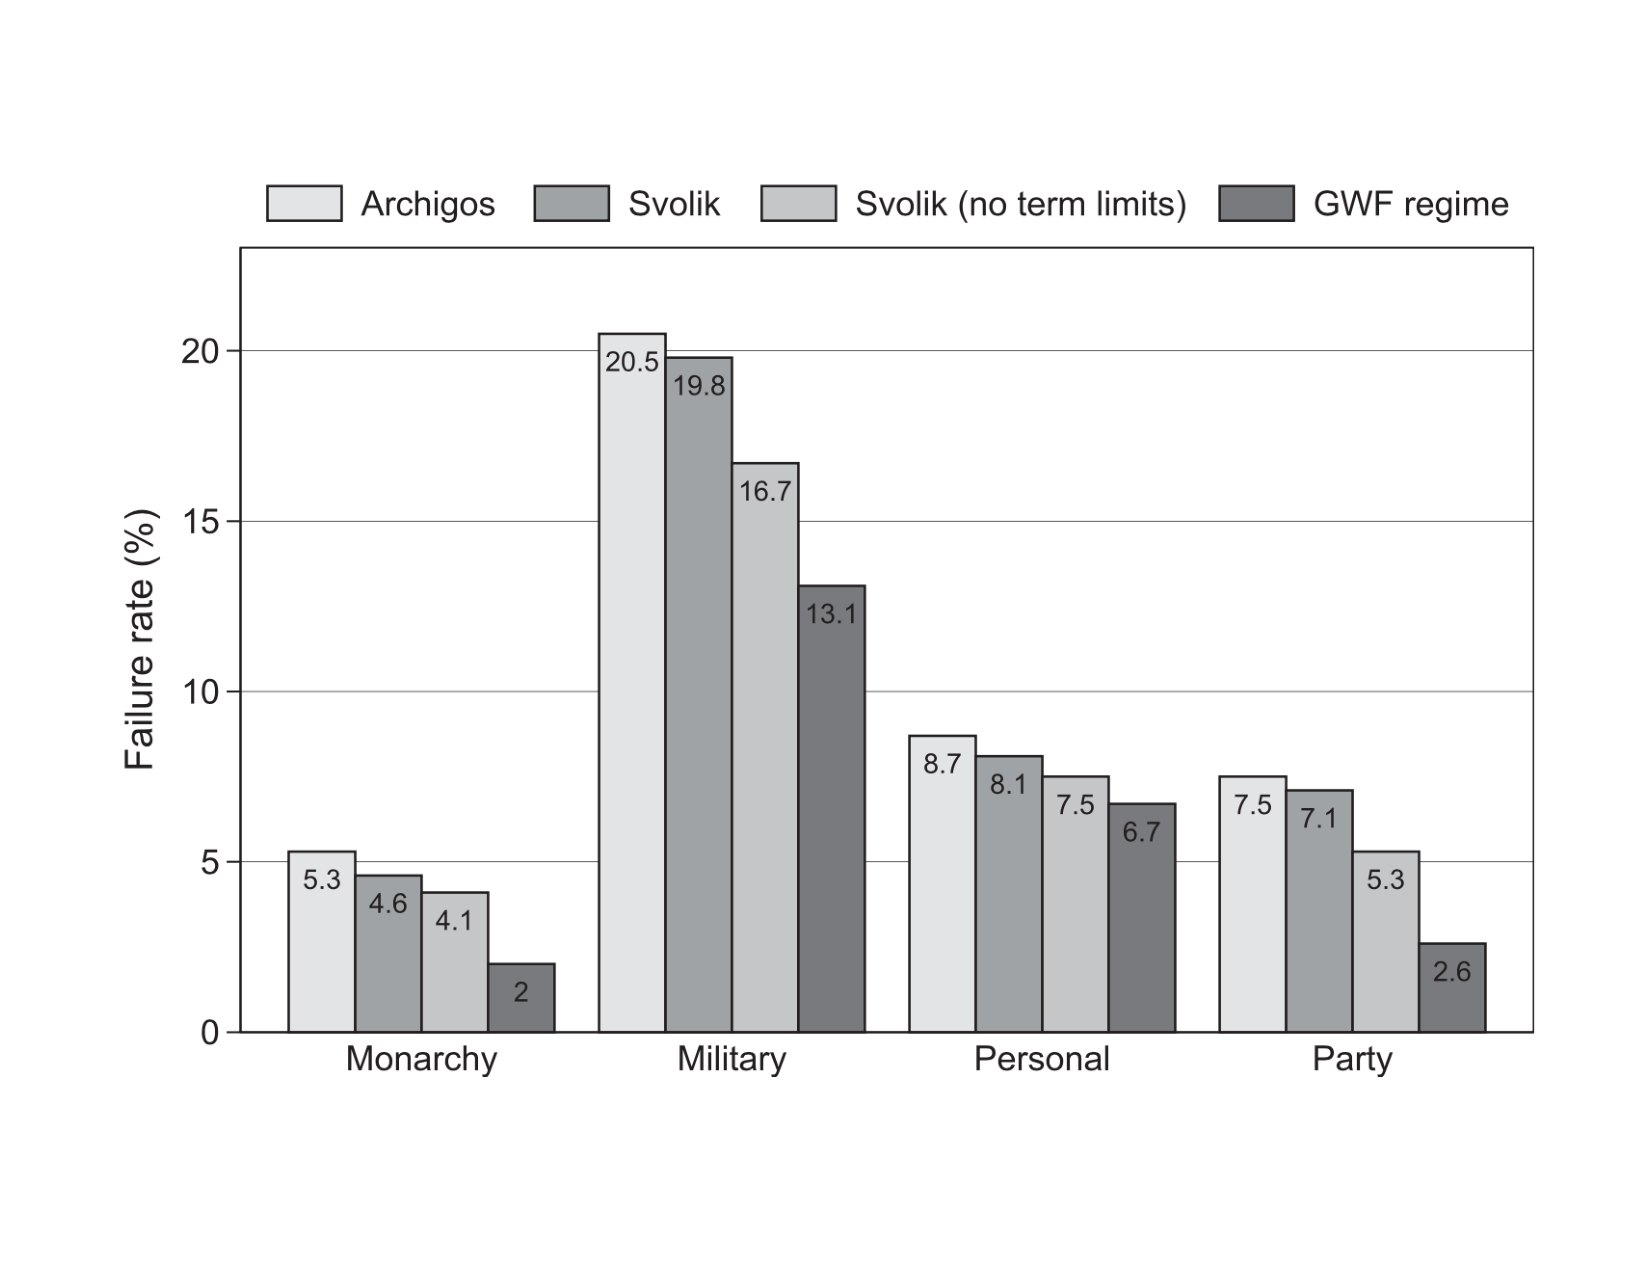
\includegraphics[scale=0.32]{Figs/GWF/survival}
	\end{figure}
	\pause
	\begin{itemize}
	\item Military regimes are most prone to collapse.
	\item Monarchies are more resilient than personalist regimes.
	\end{itemize}
\end{frame}

\begin{frame}{Regime types and authoritarian survival}
What explains the variation?
	\vspace{0.1cm}
	\pause
	\begin{itemize}
	\item Priority of those in power.
	\item How those in power interact with each other.
	\item Response to political and economic crisis.
		\pause
		\vspace{0.1cm}
		\begin{itemize}
		\item Succession.
		\item Economic depression.
		\end{itemize}
	\end{itemize}
\end{frame}

\begin{frame}{How authoritarian regimes survive}
	\begin{itemize}
		\item Repression and patronage
		\item Information control
		\item Nominally democratic institutions
	\end{itemize}
\end{frame}

\begin{frame}{How authoritarian regimes survive: Repression and patronage}
	\begin{figure}
	\centering
	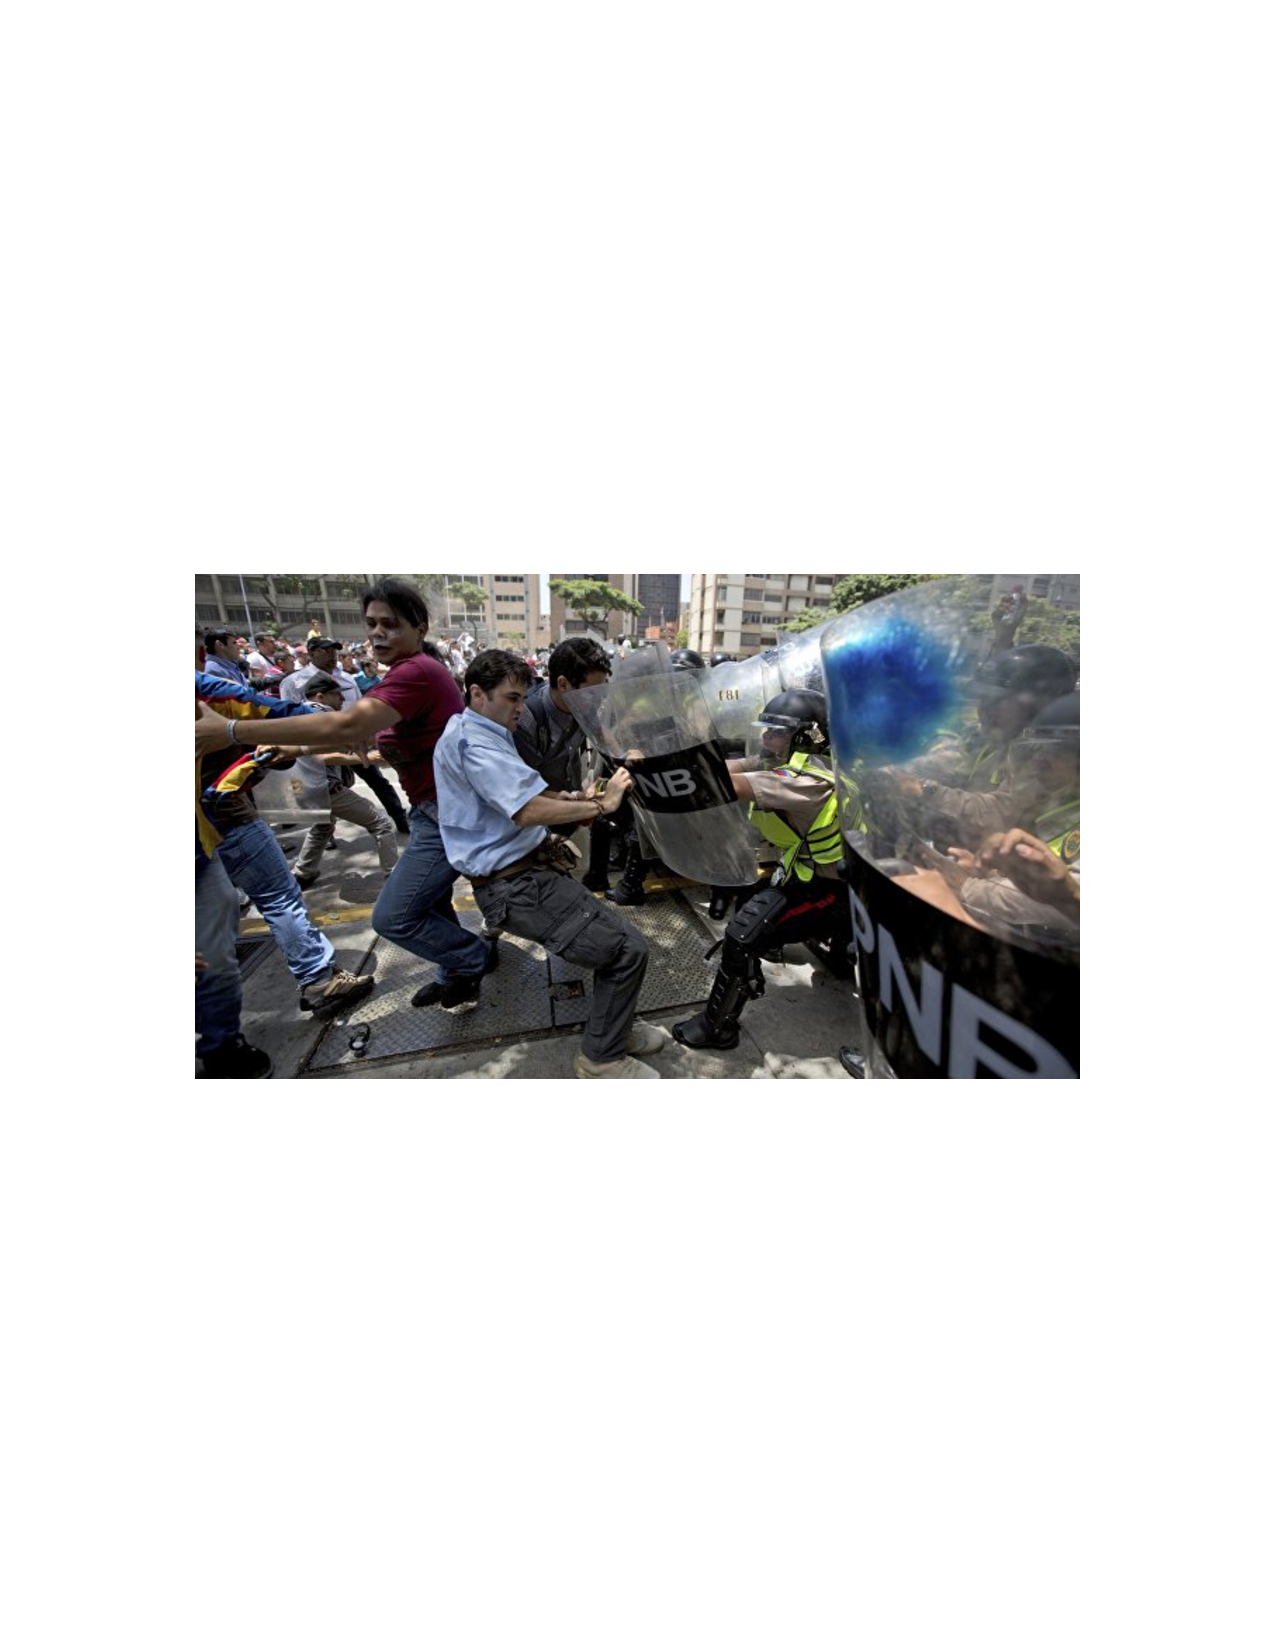
\includegraphics[scale=0.48]{Figs/repression}
	\end{figure}
	\begin{center}
	Opposition protest in Caracas, Venezuela (2017)
	\end{center}
\end{frame}

\begin{frame}{How authoritarian regimes survive: Repression and patronage}
	\begin{figure}
	\centering
	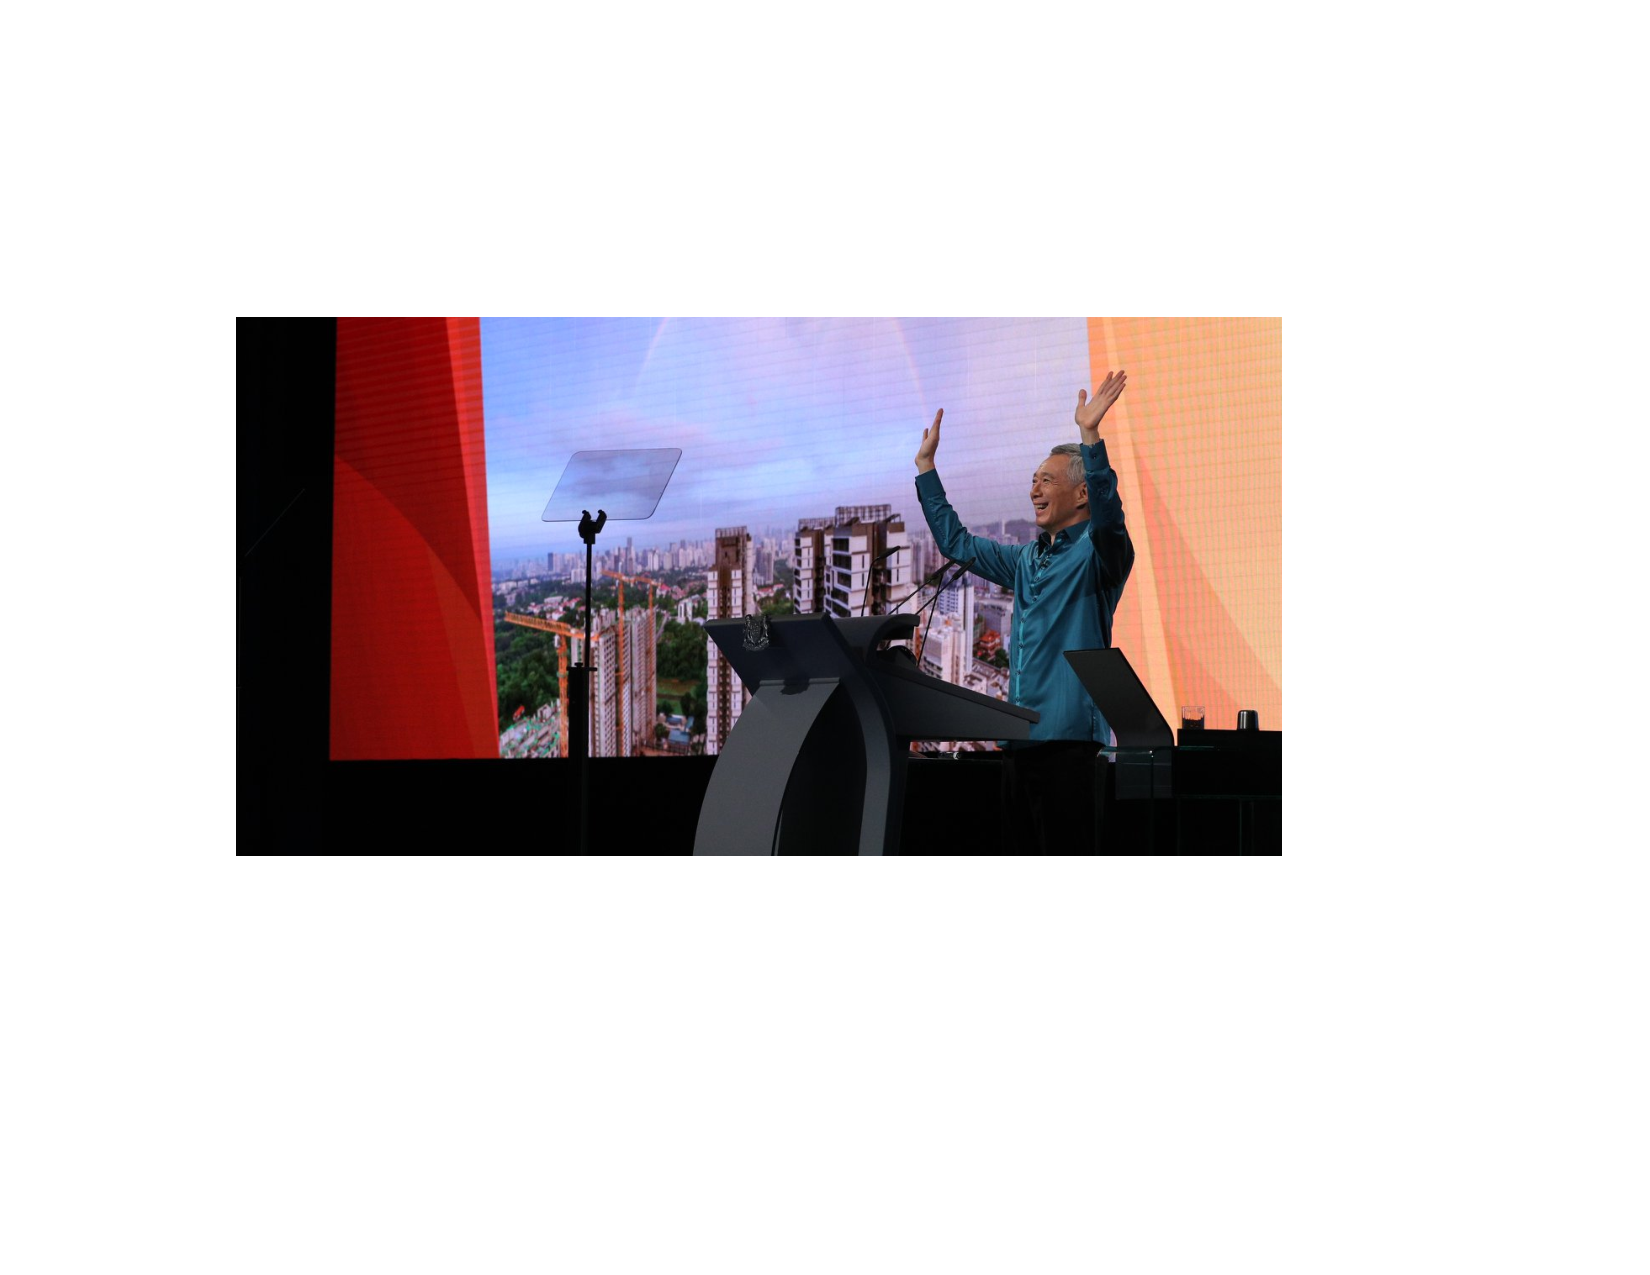
\includegraphics[scale=0.48]{Figs/lee1}
	\end{figure}
	\begin{center}
	National Day Rally in Singapore (2018)
	\end{center}
\end{frame}

\begin{frame}{How authoritarian regimes survive: Repression and patronage}
	\begin{columns}
    \column{0.5\linewidth}
	``No one should be denied medical care because they cannot afford it and that is my commitment to you. I introduced the \textbf{Pioneer Generation Package} (PGP) in 2014. Now, the Government will be rolling out the `Merdeka Package' to those in their 60s, who had just missed out on qualifying for the PGP.'' 	
    \column{0.42\linewidth}
    \centering
    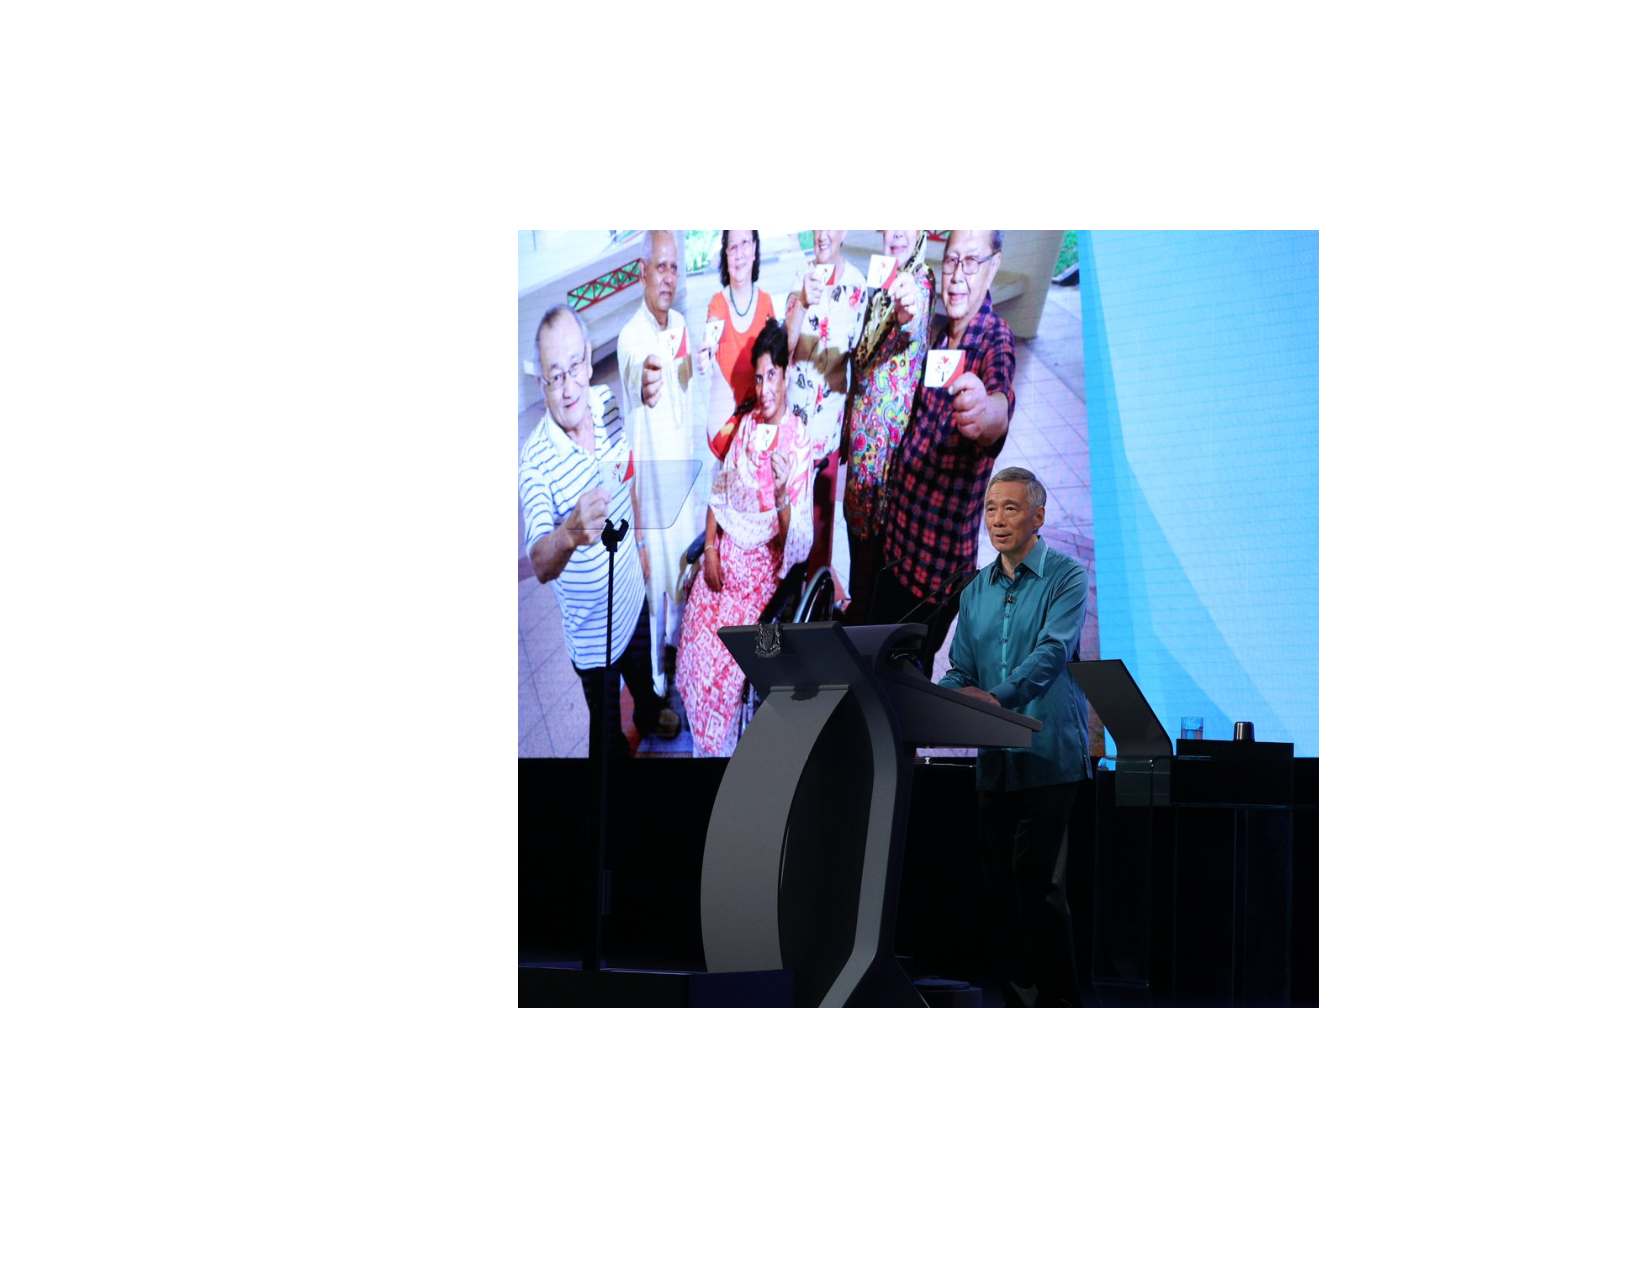
\includegraphics[scale=0.45]{Figs/lee2}
    \end{columns}
\end{frame}

\begin{frame}{How authoritarian regimes survive: Repression and patronage}
	\begin{itemize}
	\item Different targets
	\item A dilemma
	\item How oil countries remain undemocratic
	\end{itemize}
\end{frame}

\begin{frame}{How authoritarian regimes survive: Information control}
	\begin{figure}
	\centering
	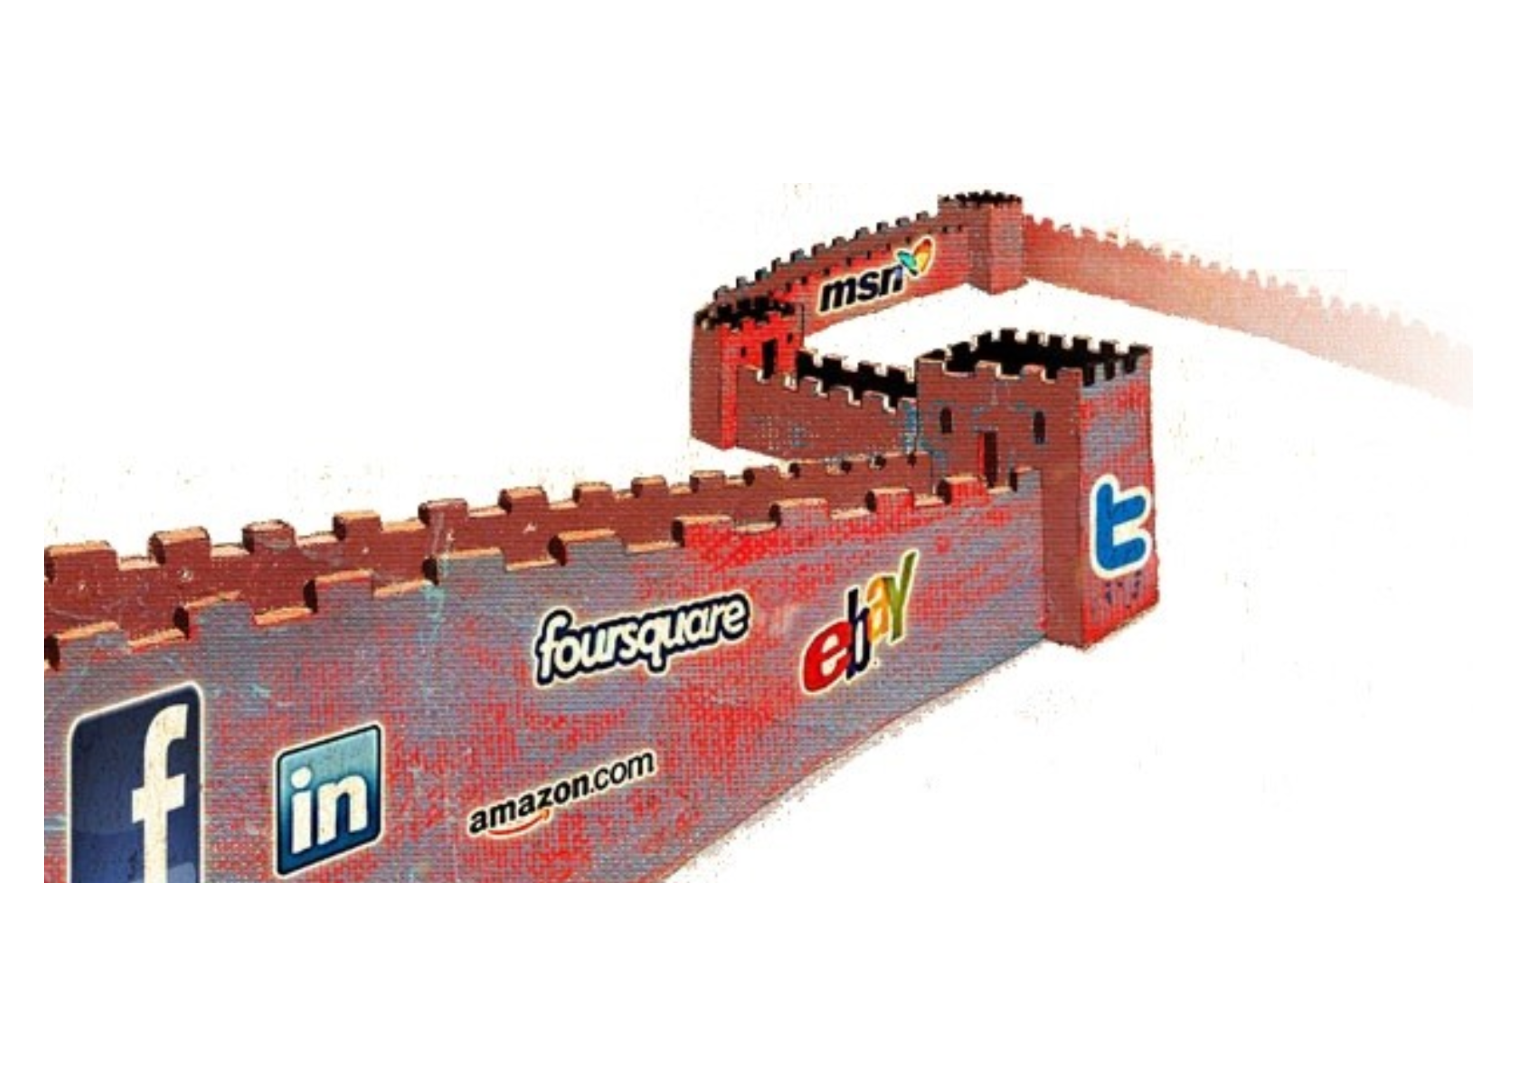
\includegraphics[scale=0.35]{Figs/firewall}
	\end{figure}
	\pause
	Strategic use of censorship?
	\begin{itemize}
	\item Getting information without fueling protests
	\end{itemize}
\end{frame}

\begin{frame}{How authoritarian regimes survive: Nominally democratic institutions}
	\begin{figure}
	\centering
	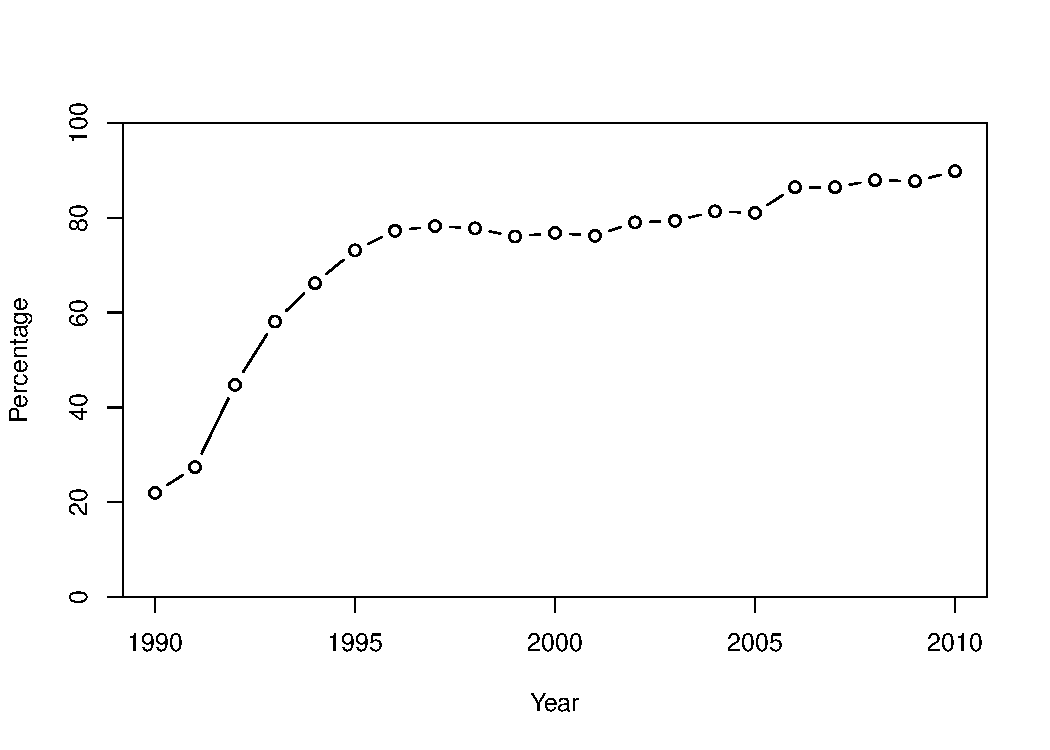
\includegraphics[scale=0.56]{Figs/election}
	\end{figure}
\end{frame}

\begin{frame}{How authoritarian regimes survive: Nominally democratic institutions}
	\begin{figure}
	\centering
	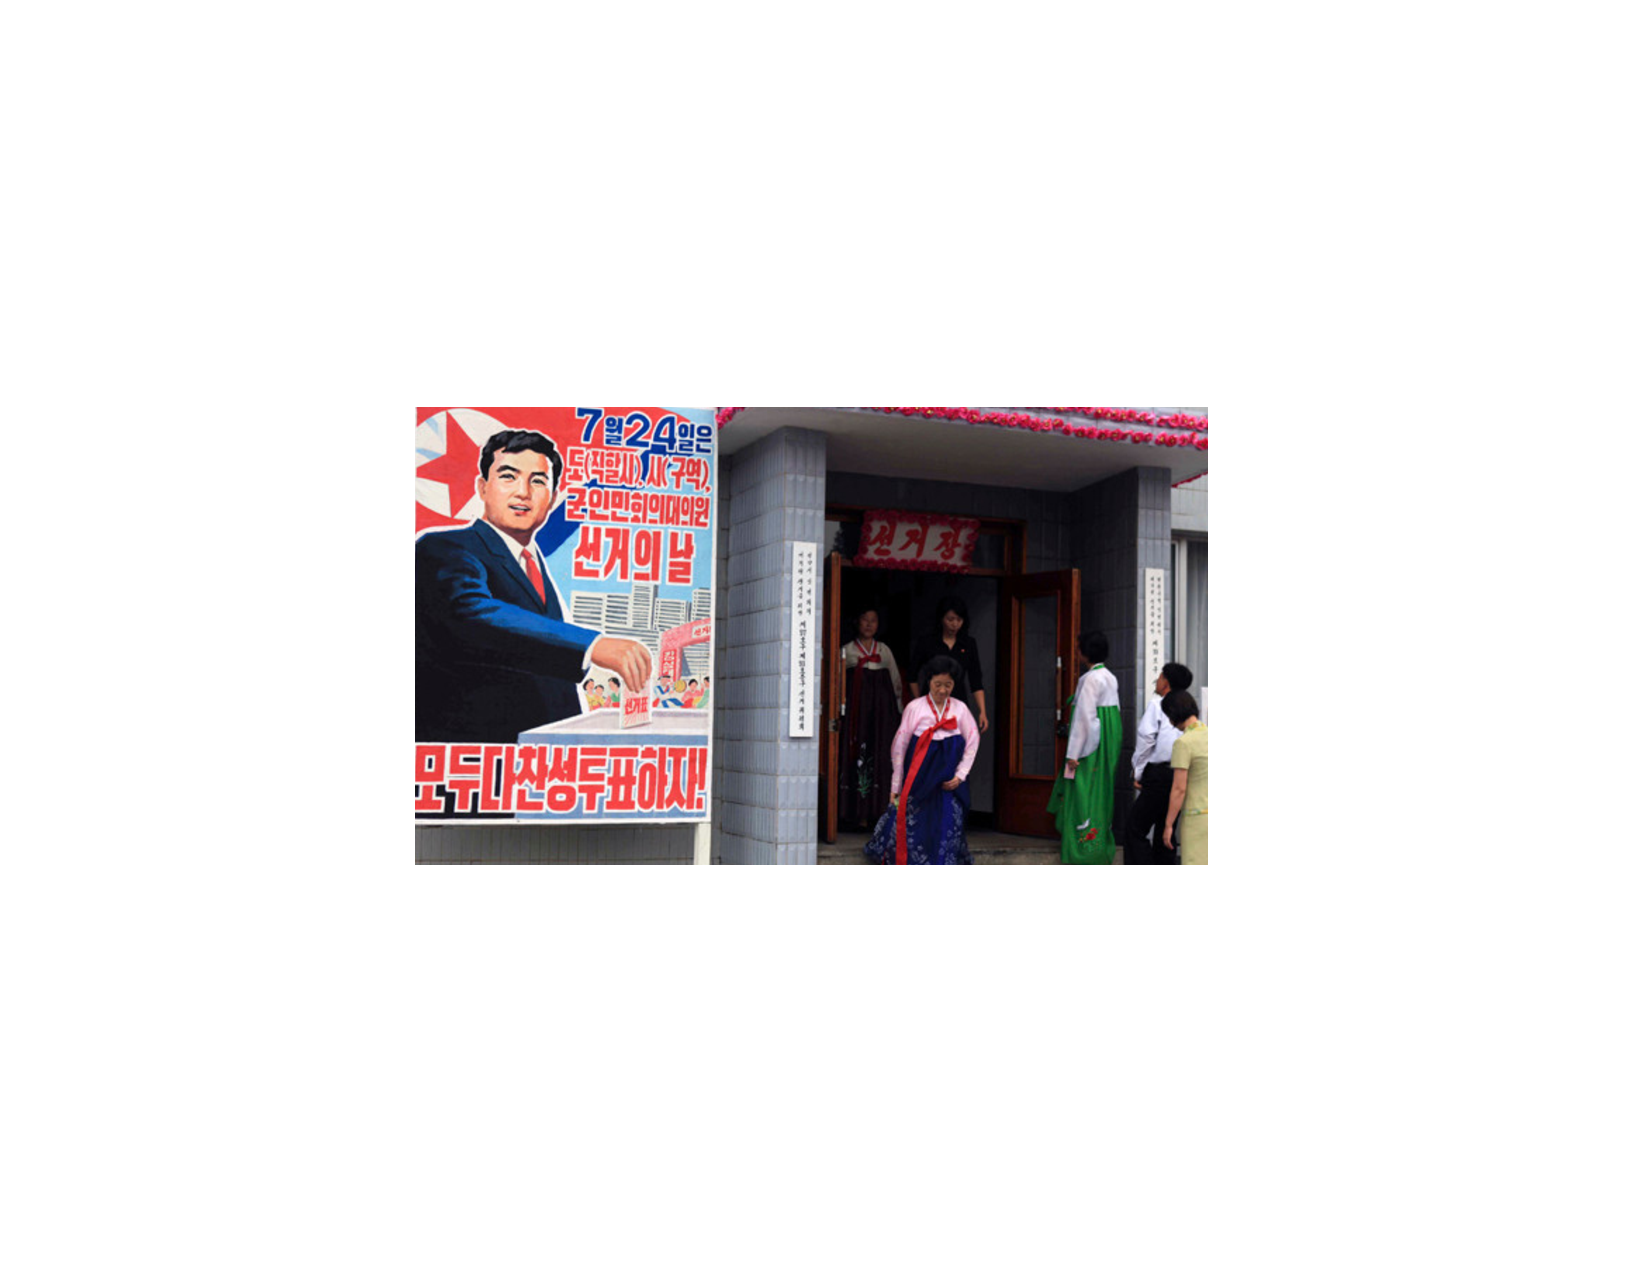
\includegraphics[scale=0.6]{Figs/nkorea}
	\end{figure}
	\begin{center}
	Election for the Supreme People's Assembly (SPA) in North Korea, March 9th 2014 
	\end{center}
\end{frame}

\begin{frame}{How authoritarian regimes survive: Nominally democratic institutions}
	\begin{figure}
	\centering
	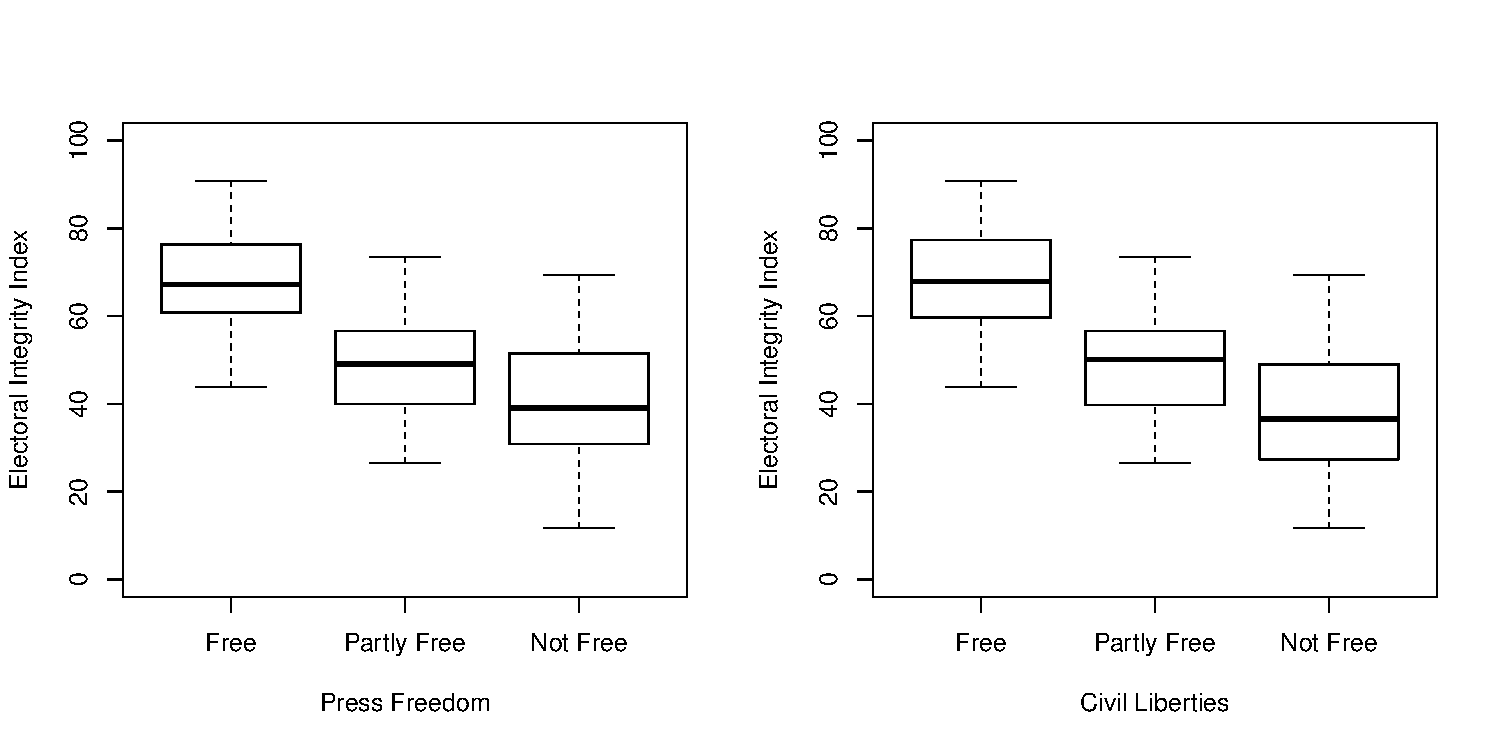
\includegraphics[scale=0.42]{Figs/pei}
	\end{figure}
\end{frame}

\begin{frame}{How authoritarian regimes survive: Nominally democratic institutions}
	\begin{itemize}
		\item Political co-optation
		\item Signaling dominance
		\item Information gathering
		\item Principal-agent problems
	\end{itemize}
\end{frame}

\begin{frame}{3-D politics: Selectorate and winning coalition}
	\begin{figure}
	\centering
	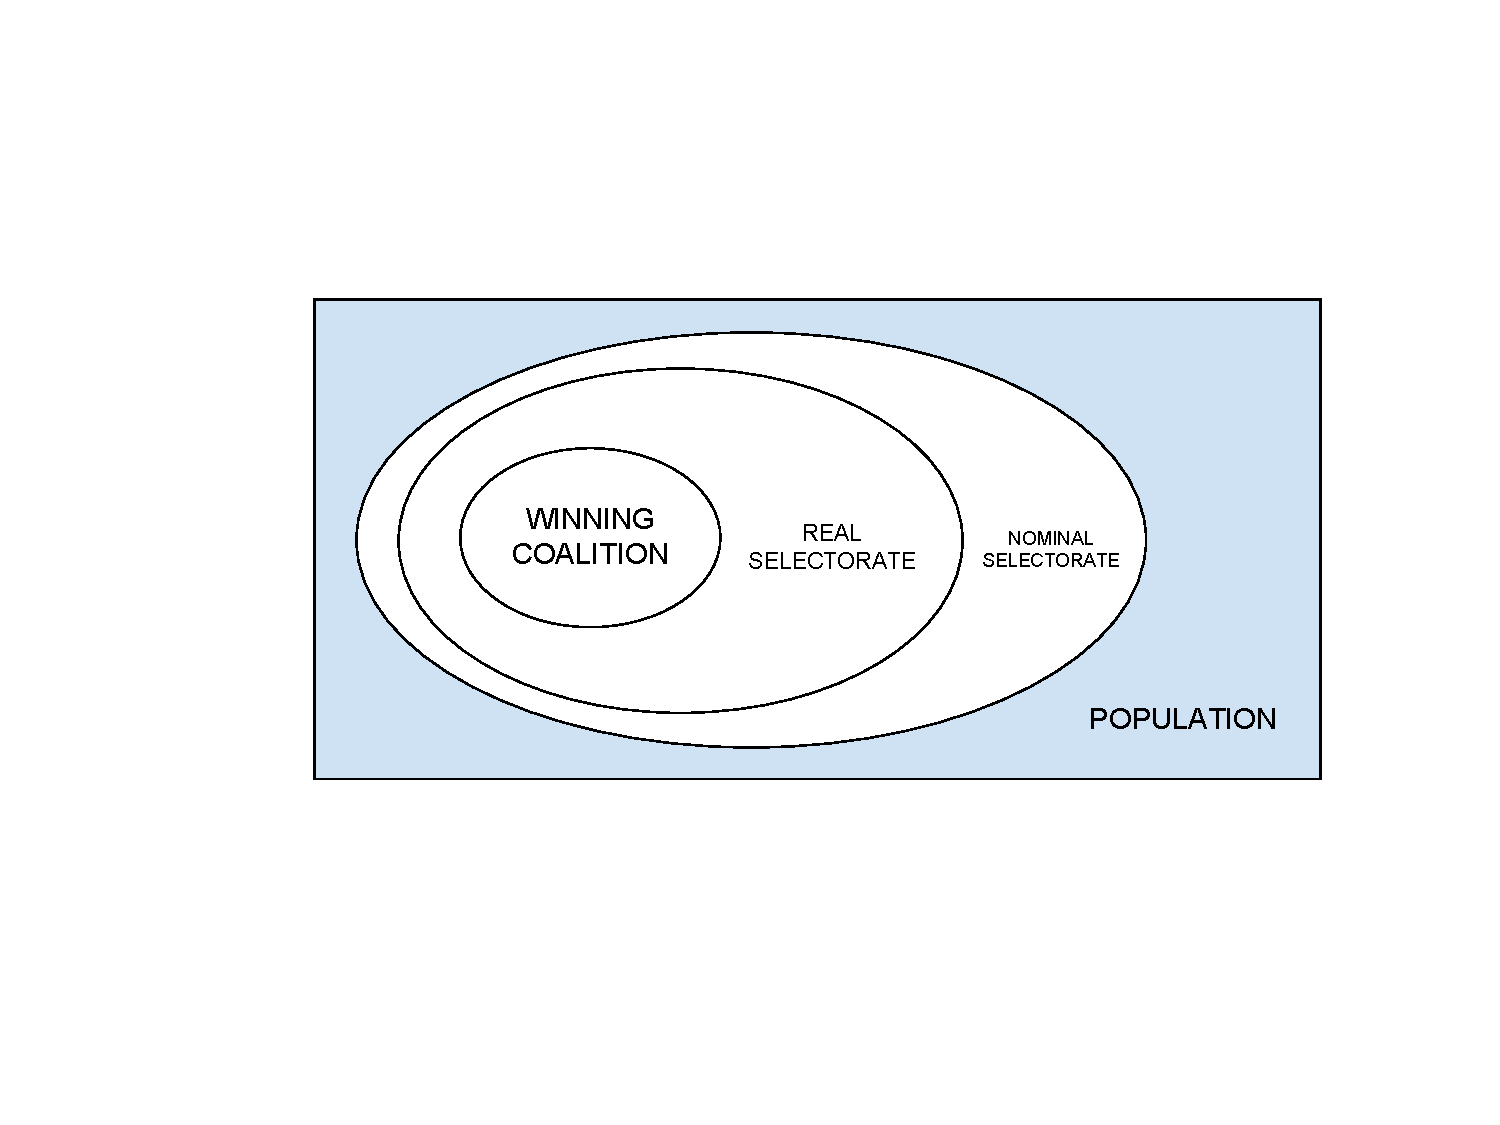
\includegraphics[scale=0.5]{Figs/selectorate}
	\end{figure}
	\pause
	\begin{itemize}
	\item Reshuffling
	\item Redistribution
	\end{itemize}
\end{frame}

\begin{frame}{Conclusion}
	\begin{itemize}
		\item No dictator rules alone.
		\item Democracy vs. autocracy?
	\end{itemize}
\end{frame}

\end{document}